%!TEX root = ../thesis.tex
%*******************************************************************************
%****************************** Third Chapter **********************************
%*******************************************************************************
\chapter{Timing Performance of the Data Acquisition System}
\label{ChapterDAQ}
% **************************** Define Graphics Path **************************
\ifpdf
    \graphicspath{{Chapter7/Figs/Raster/}{Chapter7/Figs/PDF/}{Chapter7/Figs/}}
\else
    \graphicspath{{Chapter7/Figs/Vector/}{Chapter7/Figs/}}
\fi

%********************************** %Opening  **************************************
Achieving a timing precision $\mathcal{O}$(1 ns) is a pivotal goal for the Data Acquisition (DAQ) at the Short-Baseline Near Detector (SBND) as it is essential for high precision physics analysis. 
Most importantly, the Cosmic Ray Taggers (CRTs) and PhotoMultiplier Tubes (PMTs) are the two detection subsystems with sufficient timing resolution to resolve the nanosecond bucket structure of the Booster Neutrino Beam (BNB).
Their readout electronics must have sufficient timing resolution to record the signals with a high level of precision and minimal smearing.
It is therefore important to characterise the timing performance of the readout electronics to identify areas of improvement in preparation for the nanosecond goal. 

The work undertaken to assess the timing performance of the DAQ electronics is outlined in this chapter.
An overview of the timing system at SBND is first given in Section \ref{sec4TimeRef}. 
The timing characterisation of the CRT and PMT readout electronics are detailed in Section \ref{sec4InternalClock} and \ref{sec4PMT} respectively.
Finally, Section \ref{sec5Remarks} provides some concluding remarks.

%********************************** %Second Section  **************************************
\section{Timing Reference System of the Data Acquisition}
\label{sec4TimeRef}

%short description of why need timing reference
The event building process of the DAQ relies entirely on fragment timestamps to construct a physics event, as detailed in Section \ref{sec:evb}.
The timestamp of each subsystem readout electronics must be generated with a high level of precision and synchronisation.
At SBND, the strategy is to utilise the White Rabbit (WR) timing system.
It is a collaborative project developed at the European Organisation for Nuclear Research (CERN) and is now a widely-used synchronisation solution in the scientific community \cite{WR_paper}.
The WR has the capability to offer fully deterministic time transfer with sub-nanosecond accuracy over distances exceeding 80 km.
The application of the WR timing system at SBND for time transferring and timestamping is detailed in Section \ref{subsec41TimeRef} and Section \ref{subsec42TimeRef} as follows.

%SBND aims to achieve timing precision of the DAQ hardware and software readout components in the order of nanoseconds to fully leverage the physics capabilities.

%description of WR timing 
%The system is currently installed in both the ICARUS and SBND detector buildings.
%The installation serves the dual purpose of ensuring timing precision within a single experiment as well as timing synchronisation across the two experiments. 

\subsection{Time and Frequency Transfer to Subsystems}
\label{subsec41TimeRef}

%Time Transfer Concept
Fig. \ref{fig:timeTransfer} provides an overview of the WR timing system at SBND.
Starting from the first column of the figure is the Grandmaster switch.
It distributes time and frequency to all other slave WR switches within the WR network via optical links.
The WR switch has dynamic calibration and thus, is a very reliable and robust delivery system.
The system ensures that the Pulse Per Second (PPS), which is of 1 Hz, from all slave switches are aligned to the Grandmaster's PPS with sub-nanosecond accuracy.
The Grandmaster switch is also connected to an atomic clock locked to a global navigation satellite system.
As a result, the time and frequency distributed by the WR system are derived from the International Atomic Time (TAI) and the Coordinated Universal Time (UTC) format.

At SBND, there are two slave WR switches, as shown in the second column labelled \textit{Servers Hosting Slave Switches}.
Each slave switch server hosts a different module of Field programmable gate arrays Mezzanine Card (FMC).
The first server contains two SVEC-FD modules, which are Fine Delay (FD) cards carried by Simple VME FMC Carrier (SVEC).
The second server hosts a single SPEC-TDC module, a Time to Digital Converter (TDC) card carried by a Simple PCIe FMC Carrier (SPEC).
The usage of SVEC-FD modules is discussed here, whilst the usage of the SPEC-TDC is discussed in Section \ref{subsec42TimeRef} next.

\begin{figure}[b!] 
\centering    
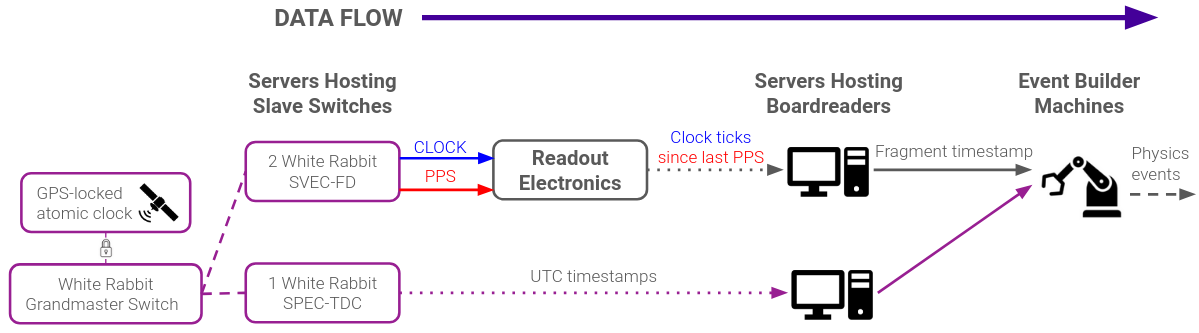
\includegraphics[width=1.0\textwidth]{time_transfer}
\caption[White Rabbit Timing System Distribution]{
Distribution of the White Rabbit timing system.
}
\label{fig:timeTransfer}
\end{figure}

SVEC-FD modules are high precision pulse generators, with 10 ps resolution when used within a WR network \cite{WR_paper}.
They are used to generate frequencies sent to readout electronics to ensure timing synchronisation across all subsystems of the DAQ.
There are two types of frequencies: (1) clock as shown by the blue arrow and (2) PPS as shown by the red arrow in Fig. \ref{fig:timeTransfer}.

The clock signal provides a \textit{metronome frequency} customised for each readout hardware's internal clocks.
This signal behaves as the master clock that the internal clocks of readout electronics can latch onto, thereby maintaining their accuracy and stability over time.
The PPS signal provides the \textit{same reference frame} for all readout electronics in the DAQ.
All internal clock counters of readout electronics reset upon the arrival of a PPS and thus share the same reference frame as the PPS.
Details of the PPS and clock distribution are provided in Appendix \ref{appendix_timing_dist}.

Raw data sent from the readout electronics to computer servers, as shown by the dotted grey arrow, contains timing information regarding the arrival time of the trigger at the readout.
The timing information at this stage is only the number of clock ticks since last the PPS arrived, and therefore, does not contain sufficient information for event building across multiple subsystems.

To facilitate event building, raw data is packaged into \textit{fragments}, previously detailed in Section \ref{sec:evb}.
The fragment timestamp is in the UTC format, which is defined as the number of seconds since the Unix Epoch on the 1st of January 1970.
This is the \textit{universal} reference frame and allows for direct comparison of fragment timestamps from different subsystems required by event building.
The number of seconds is generated by the computer servers under the network time protocol with a precision level $\mathcal{O}$(100 ms).

The nanosecond-level of precision of fragment timestamps are derived from the number of clock ticks since the last PPS, generated by internal clocks of each readout electronics.
They are converted to the number of nanoseconds since the last whole second using the tick-to-time conversion.
This level of precision of fragment timestamp necessitates the event building process, as well as, is stored for downstream reconstruction and analysis.

\subsection{Precise Timestamping}
\label{subsec42TimeRef}

%Precision Timestamp concept
%description of SPEC TDC
Also shown in Fig. \ref{fig:timeTransfer}, another component of the WR timing system is the SPEC-TDC module.
This module timestamps signals with a precision of 700 ps, and outputs timestamps in the UTC format.
The timestamps can be acquired by the DAQ and be built within a physics event, as shown by the dotted and solid purple arrows. 

% SPEC TDC
At SBND, SPEC-TDC is employed to timestamp the arrival time of important signals, recording additional timing information on top of the Time Projection Chamber (TPC), Photon Detection System (PDS) and Cosmic Ray Tagger (CRT) data.
This timing information can be leveraged for different physics applications.
For instance, it can be used to characterise the timing resolution of the readout electronics.
The recorded timestamps can be also used to derive the correction for hardware synchronisation or enable an alternative method to reconstruct the timing of a physics event. 

Fig. \ref{fig:SPECTDC} shows the five signals input to the SPEC-TDC. 
Two beam signals, shown in blue, provide the status of the BNB.
The first one is the Booster Extraction Signal (BES), which is an early warning indicating when protons are extracted in the Booster.
The second one is the Resistor Wall Monitor (RWM), which measures the time and intensity of protons striking the target.
The RWM signal arrives at the SBND detector building almost instantaneously with the beam itself due to the close proximity of SBND to the target.
Additionally, two trigger signals, shown in green, are recorded to monitor the DAQ synchronisation with respect to the triggers. 
These include flash and event triggers (See Section \ref{sec:sbnd_trigger}).
Finally, clock reset signals for the CRT readout electronics are recorded in the last channel as shown in pink. 

\begin{figure}[hb!] 
\centering    
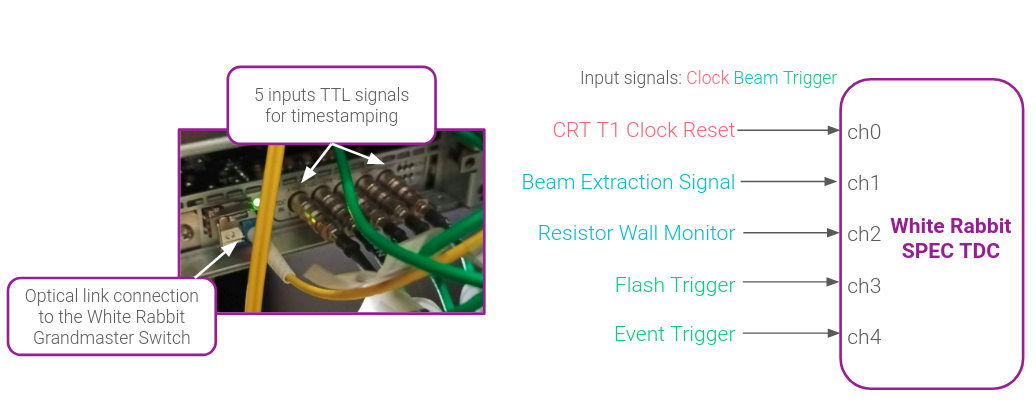
\includegraphics[width=1.0\textwidth]{SPEC_TDC}
\caption[SPEC-TDC Module and Its Input Signals]{
The SPEC-TDC module installed at SBND (left) and signals input to the module for timestamping (right).
}
\label{fig:SPECTDC}
\end{figure}

Two applications of the SPEC-TDC to characterise the timing precision of the readout electronics were explored for CRT and PMT readout electronics in Sections \ref{sec4InternalClock} and \ref{sec4PMT} respectively.
For the CRT, an alternative timing reconstruction was also derived using the timing information recorded by the SPEC-TDC.
For the PMT, SPEC-TDC timestamps helped validate the timing synchronisation across multiple digitisers. 

%Upon receiving this signal, the CRT readouts reset the counters of its internal clocks.
%Thus, monitoring this signal provides direct measurement of the resolution of the CRT readouts clocks.
%This study was carried out by the author and is described in section \ref{sec4InternalClock}.

%Referencing back to Fig. \ref{fig:daqOverview}, an event contains two types of trigger: a single Event trigger and multiple Flash triggers. 
%Both types of triggers are issued relative to the beam, such that the PTB only issues triggers within the beam spill window.   
%The recorded trigger timestamps can be cross referenced to the beam timestamps, and thus, enabling monitoring of the triggering synchronisation to the beam in real-time.

%Following Fig. \ref{fig:SPECTDC}, one application of the SPEC-TDC is to synchronise the DAQ system with respect to the beam.
%The delay between the BES and the RWM signal is approximately 333 us.
%Recording the timestamps of these beam signals provides valuable tools for various monitoring purposes. 
%such that it contains the last whole second in UTC format and the number of nanoseconds since the last whole second.
%Thus, the timestamps are in the same time frame of reference with respect to the PPS signal.
%Moreover, the SPEC-TDC also has its own boardreader so that the recorded timestamps can be built within an event, and available for downstream analysis.
%Usage
%SPEC-TDC capabilities of high precision timestamping can be leveraged for physics application.
%Recording both the timestamps of the beam and trigger signal in a single event opens up venues for various physics applications. 
%One example is the characterisation of timing resolution the DAQ hardware readouts, by directly comparing the timestamps produced by the hardware against the timestamps of the SPEC-TDC given that both share the common time reference to the PPS signal.
%Furthermore, it provides useful timing information for downstream analysis, for example, applying timing correction for hardware resolution and providing alternative method for event timing reconstruction. 
%The SPEC-TDC applications are to be explored in the future includes nanosecond timing reconstruction, allowing for physics application such as cosmics rejection and physics searches between neutrino bucket.

%The author has worked extensively on installing, testing and calibrating the SPEC-TDC over her visits at Fermilab.
%The  conducted work included the hardware installations of the SPEC-TDC, by testing out two different PCIe connections on two different servers. 
%One server can hold the SPEC-TDC horizontally whilst the other can hold the SPEC-TDC vertically. 
%The latter was chosen due to better structural support and ventilation to host the SPEC-TDC.
%The software boardreader of the SPEC-TDC also had some improvements implemented by the author, namely, better timestamp correction and higher data processing rate.
%The calibration work included measuring a constant offset introduced by the SPEC-TDC hardware to be 58 ns.

%********************************** %Second Section  **************************************
\section{Timing Performance of Front End Board Modules}
\label{sec4InternalClock}

%Thus, the DAQ workflow places a vital importance on the internal clocks of each hardware readout, which are further explored in section \ref{sec4InternalClock} and section \ref{sec4PMT} for the CRTs and PMTs electronics respectively.

This section provides a description of the characterisation of the timing performance of the CRT readout electronics, Front End Board (FEB) modules, in Section \ref{sec:crt_time_precision} and an alternative timing reconstruction in Section \ref{sec:crt_time_alternative}.

\subsection{Evaluation of Internal Clock Resolution}
\label{sec:crt_time_precision}

%Clock description
The readout electronics of CRTs are FEB modules as detailed in Section \ref{sec:readout}.
Here, the focus is on the precision of the internal clocks of FEB modules. 
Internal clocks of FEB modules are TDC units with a coarse counter of 4 ns per tick (250 MHz frequency) \cite{crt_note}. 
A high resolution time interpolation method is implemented within the TDC clock cycle to improve the counter to 1 ns per tick \cite{crt_clock}.

There are two internal clocks per FEB module.
The first one is referred to as \textit{T0 clock}, which is reset by the PPS signal, therefore its \textit{T0 timestamps} share the same PPS reference frame as all other readout electronics.
The second internal clock is referred to as \textit{T1 clock}, which is reset by the BES signal of the frequency $\sim 5$ Hz. 
It produces \textit{T1 timestamps}, referencing to the BES signal coincident with the beam arrival time.
In addition, FEB modules timestamp the arrival time of reset signals, whether a PPS or a BES, and store the timestamps as \textit{T0 or T1 clock reset events}.
Reset events are timestamped by both the T0 and T1 clocks, and therefore have both T0 and T1 timestamps.
%In other words, the T0 (T1) timestamp of the clock reset event is the number of ticks of the T0 (T1) clock upon receiving a reset signal.

%of the reference pulse and save it as special non-physics events, called clock reset event.
%The clock resets its counter upon receiving an input reference pulse.  
%The generated timestamp is the number of ticks since the clock last resets.
%This clock produces T0 timestamp, referencing to the PPS frame of reference.
%The generated T1 timestamp is expected to have a higher precision since the T1 clock is reset more frequently. 
%Because of this clock system, the FEB module generates two independent timestamps, T0 and T1 with respect to the PPS and BES signal, for every recorded event.
%The FEB module also records two types of clock reset event for the T0 and T1 clock.

%, of which each can be reset independently via external TTL signal into LEMO connections of the module.

%CRT Sharp Set Up
%Over the summer of 2022, the author has travelled to Fermilab to conduct the work on evaluating the timing resolution of the FEB module.

The work to characterise the internet clock was undertaken at Fermilab in 2022 during the commissioning of SBND.
It was conducted using a temporary setup called \textit{CRT Sharps}.
The setup was made up of two sets of CRT panels, where each set was placed upstream and downstream of the cryostat centred on the BNB.
The downstream setup is photographed in Fig. \ref{fig:crtSharps}, showing 4 CRT panels arranged perpendicular to each other.
Each panel was read out by a FEB module, totalling 8 FEB modules with 4 upstream and 4 downstream.
The CRT Sharps was commissioned during the period at which the BNB beam was on so that it functioned as a beam telescope.
The triggering condition was to have signal coincidences between the upstream and downstream panels during the beam spill to record events produced by muons from neutrino interactions.

\begin{figure}[htbp!] 
\centering    
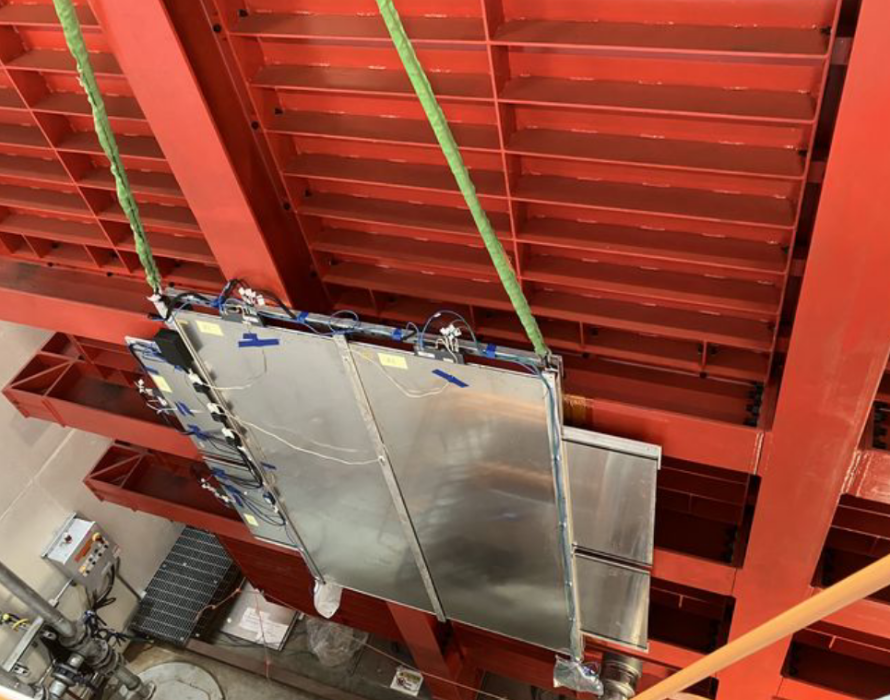
\includegraphics[width=0.6\textwidth]{crt_sharps}
\caption[CRT Sharps Setup]{
Downstream panels of the CRT Sharps installed on the downstream wall of the SBND cryostat. 
}
\label{fig:crtSharps}
\end{figure}

%T0 Clock
%As previously described, the FEB can store the timestamps of clock reset events, which are the timestamps at which the input reference signals arrive at the FEB module.
% corrected for cable length differences.

The T0 clock is characterised using T0 timestamps of T0 clock reset events.
To measure the clock variation, one can simply compare these timestamps with respect to a whole second.
An example is shown in Fig. \ref{fig:UpstreamT0StabilityCombinedBoard79} for a single FEB module numbered 79.
The left plot shows the timestamp variation with respect to the event number to check for clock stability over a period of time.
The right plot is a 1D histogram to check for the spread of the distribution.
The standard deviation of this distribution is a direct measurement of the T0 clock variation.
It is 2.37 ns with a mean of -1.89 ns, indicating that the FEB module 79 consistently received the PPS signal every second to reset its T0 clock.
This measurement was repeated for all 8 FEB modules of the CRT Sharps.
The T0 clock resolution was found to be $\mathcal{O}$(2 ns), consistent across all FEB modules.

The characterisation of the T1 clock is less trivial since its T1 timestamps do not share the same reference frame with any other readout electronics.
The only direct comparison is via T0 timestamps, which contain the T0 clock resolution. 
T0 timestamps of T1 clock reset events were compared against the SPEC-TDC timestamps of the BES signal since they both measured the same signal and reference to the PPS.
The comparison was motivated since the SPEC-TDC has a higher precision than FEB clocks, 700 ps compared to $\mathcal{O}$(1 ns).

%When this happeThe variation of T0 timestamps of T1 clock reset events, or BES signals, as compared to the SPEC-TDC is shown in Fig. \ref{fig:UpstreamT1StabilityCombinedBoard79} for the FEB module 79.
%ns, the FEB modules can flag these events and their timestamps need to be invalidated.

The left plot of Fig. \ref{fig:UpstreamT1StabilityCombinedBoard79} shows the variation of T1 clock with respect to the event number, indicating that the FEB module 79 regularly received BES signals to reset its T1 clock.
The right plot shows the 1D histogram of the variation.
The standard deviation here is not a direct measurement of the T1 clock resolution.
It is expected to be lower than the T0 clock resolution since the T1 clock is reset more frequently at $\sim$5 Hz.
The standard deviation is smaller at 1.95 ns and the mean is closer to 0 at -0.443 ns.
This measurement was carried out for all FEB modules and the same results were observed.

\begin{figure}[ht!] 
\centering    
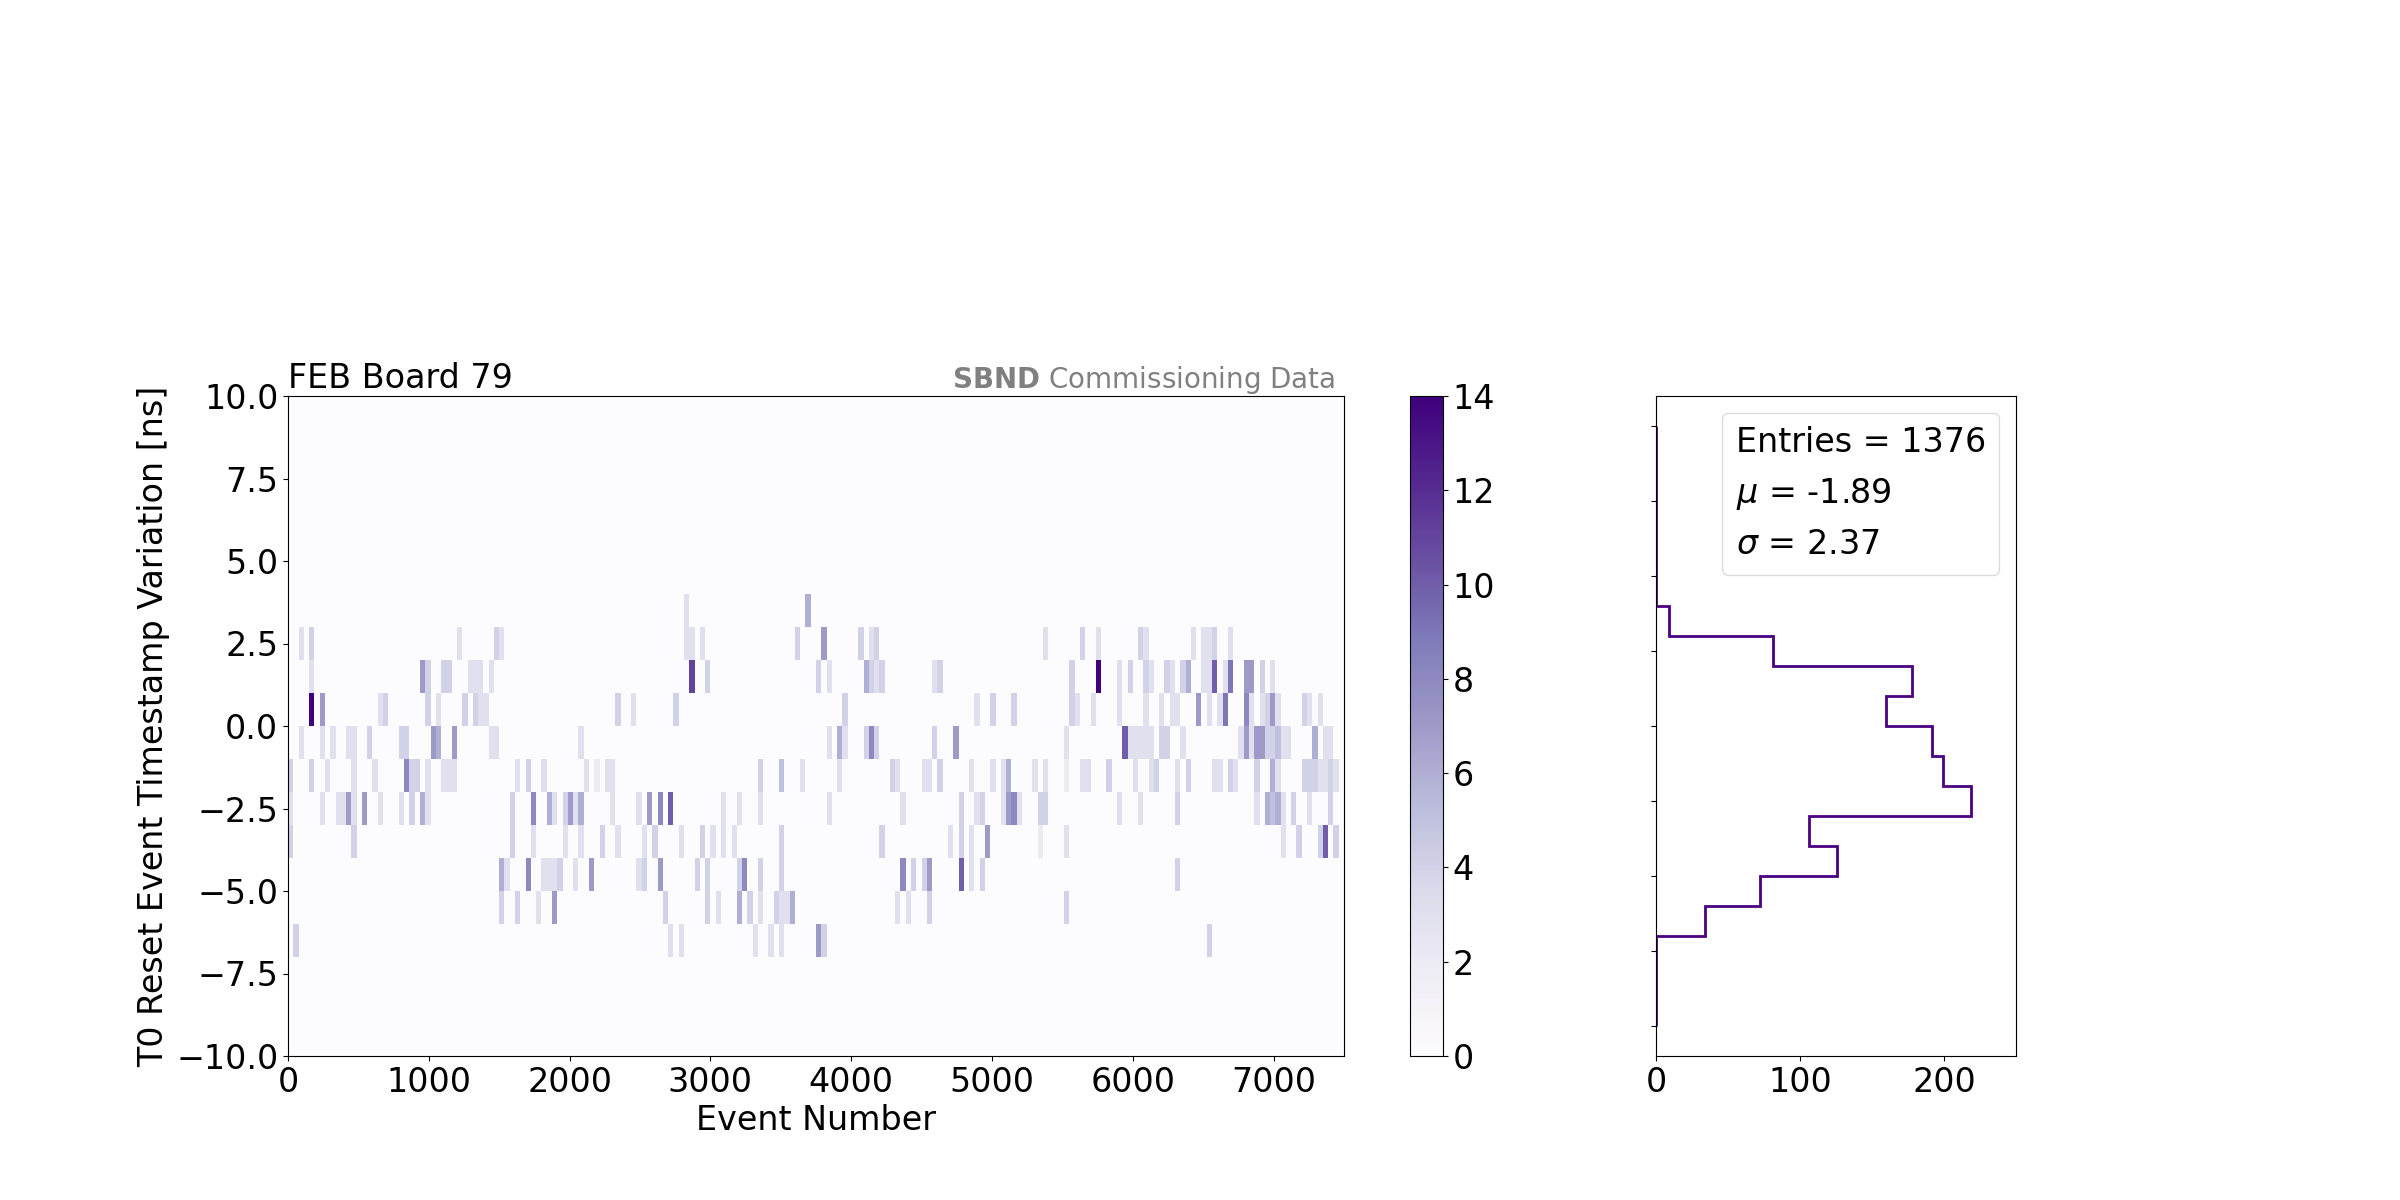
\includegraphics[width=0.85\textwidth]{upstream_T0stability_combined_board79}
\caption[Variation of T0 Timestamps of T0 Clock Reset Events Against Event Number]{
Variation of T0 timestamps of T0 clock reset events with respect to a whole second as a function of event numbers.
}
\label{fig:UpstreamT0StabilityCombinedBoard79}
%\end{figure}
%\begin{figure}[t!] 
\centering    
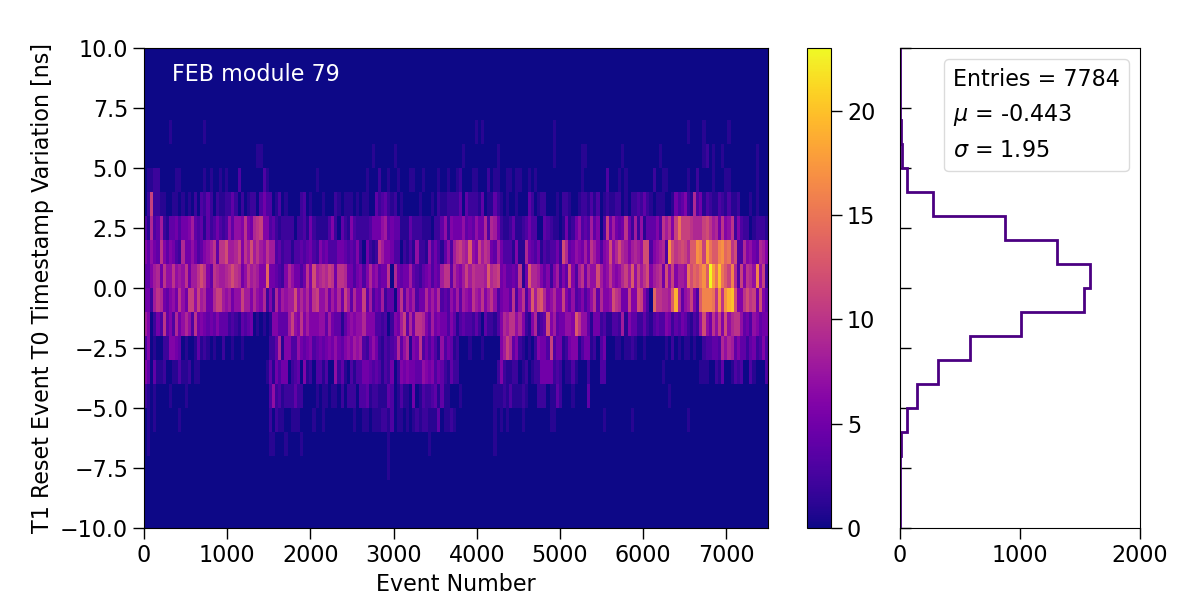
\includegraphics[width=0.85\textwidth]{upstream_T1stability_combined_board79}
\caption[Variation of T0 Timestamps of T1 Clock Reset Events Against Event Number]{
Variation of T0 timestamps of T1 clock reset events with respect to the SPEC-TDC's recorded timestamp of the BES signal as a function of event numbers.
}
\label{fig:UpstreamT1StabilityCombinedBoard79}
\end{figure}

T1 clock reset events also provide a method to monitor the drift of the T0 clock.
By plotting the variation of T0 timestamps of T1 clock reset events as a function of the T0 timestamps, it enables the monitoring of the T0 timestamp precision with respect to when it is generated in the clock cycle.
An example is shown in Fig. \ref{fig:Board79T1Drift2d} for the FEB module 79.
Early in the clock cycle, when T0 timestamps are close to 0 ns, small variations within 2 ns can be seen.
However, later in the clock cycle, when T0 timestamps are close to a whole second, larger variations up to 7 ns occur.
This demonstrates that the precision of T0 timestamps depends on at which point in the clock cycle they are generated.
It is also possible that the T0 clock counter can overflow, resulting in meaningless T0 timestamps.
This clock drift behaviour is expected to be more prevalent with the T0 clocks than the T1 clocks due to the lower reset frequency.

\begin{figure}[hb!] 
\centering    
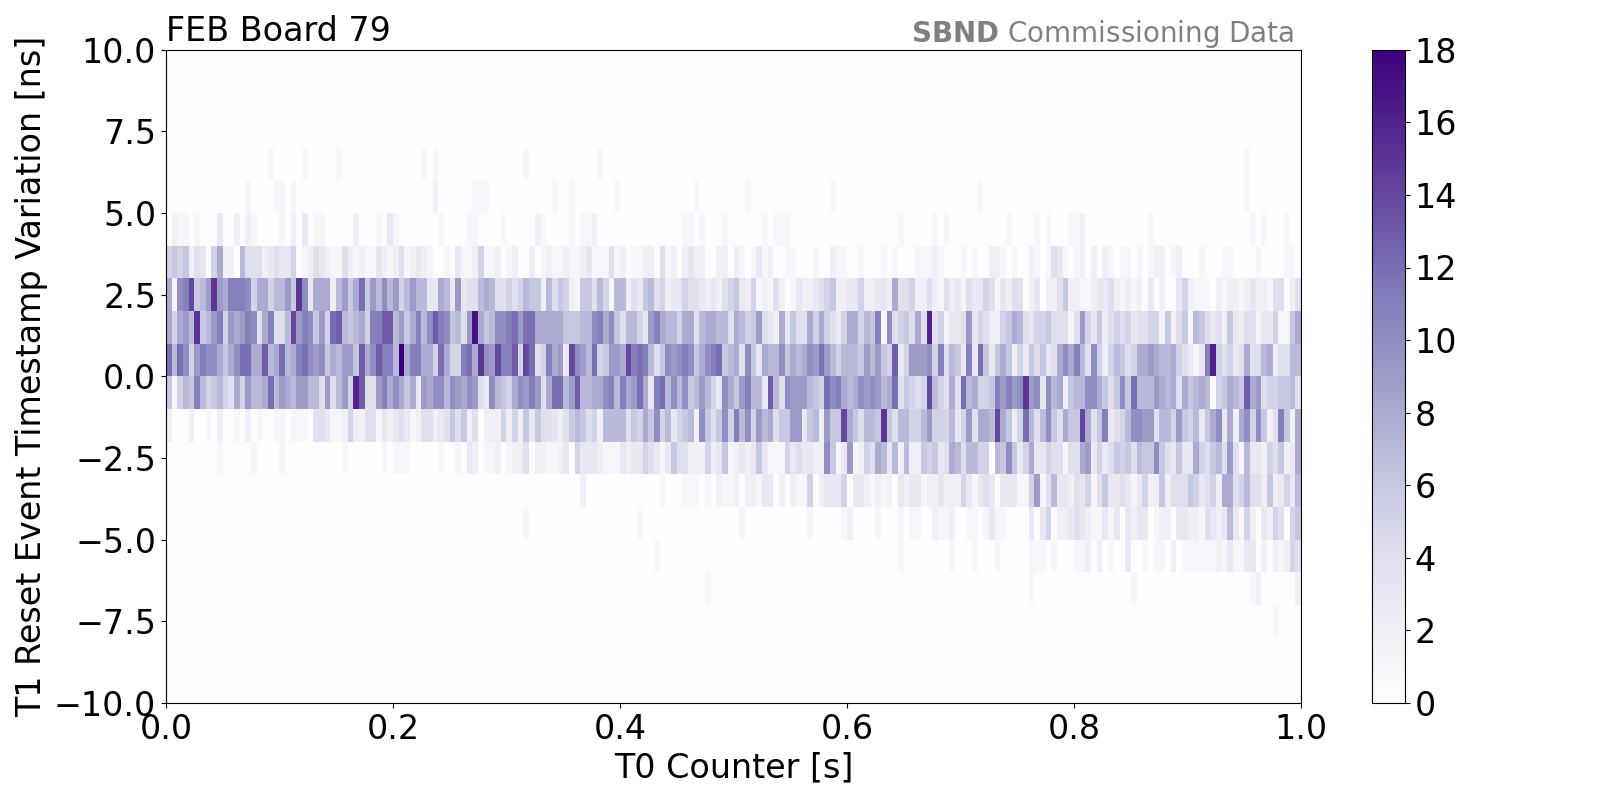
\includegraphics[width=0.70\textwidth]{board79_T1drift_2d}
\caption[Variation of T0 Timestamps of T1 Clock Reset Events Against T0 Timestamp]{
Variation of T0 timestamps of T1 clock reset events as a function of T0 timestamps. 
}
\label{fig:Board79T1Drift2d}
\end{figure}

These plots are useful diagnostic tools to characterise the timing of the FEB modules, including monitoring the magnitude and stability of the T0 and T1 clocks as well as the drift of the T0 clock.
It is important to note that the T0 and T1 clocks of the FEB can potentially vary with time, and they are very sensitive to external noises. 
The plots were reproduced during the CRT installation as apart of the quality control procedure to track the clock stability and resolution of the FEB modules.

\subsection{Alternative Timing Reconstruction}
\label{sec:crt_time_alternative}

%Having the SPEC-TDC also opens up opportunities for alternative timing reconstruction method. 
The SPEC-TDC can also provides an alternative timing reconstruction method for events recorded by CRTs.
The study here was performed using a data set recorded by the CRT Sharps consisting of $\sim$9000 beam events. 
CRT 2D hit time was reconstructed from coincidental hits of 2 cross scintillator strips, and corrected for cable and propagation delay.
CRT hit time T0 was reconstructed using the T0 timestamp whilst the CRT hit time T1 was reconstructed using the T1 timestamp. 
Commonly, the timing reconstruction of CRT data only uses the CRT hit time T1 in reference to the beam, as previously shown in Fig. \ref{fig:CRT2017}, Section \ref{sec4BNB}.
Here, the timing reconstruction using CRT hit time T0 instead is presented.

Firstly, the beam spill was reconstructed as shown in Fig. \ref{fig:topHat_T1} and \ref{fig:topHat_T0} using CRT hit time T1 and T0 respectively.
The beam spill in Fig. \ref{fig:topHat_T1} was plotted directly using CRT hit time T1 since it is a reference to the BES signal.
The plot shows a beam excess to the cosmic background, corresponding to the BNB beam arriving 333 $\mu$s after the BES signal and lasting for 1.6 $\mu$s.
On the other hand, CRT hit time T0 is in the reference frame of the PPS and needs to be corrected to the beam arrival time to reconstruct the beam spill.
The correction was done using BES signals recorded by the SPEC-TDC, of which the timestamps are also with respect to the PPS. %corrected for cable lengths.
The beam spill structure acquired from this method shows a good agreement as shown in Fig. \ref{fig:topHat_T0}, where the same beam excess can be seen.
It is important to note that the reconstruction of the beam spill only requires a resolution $\mathcal{O}$(1 $\mu$s), which is satisfied by both the T0 and T1 clock resolution $\mathcal{O}$(2 ns).

\begin{figure}[hb!]
\begin{subfigure}[h]{0.495\linewidth}
\centering    
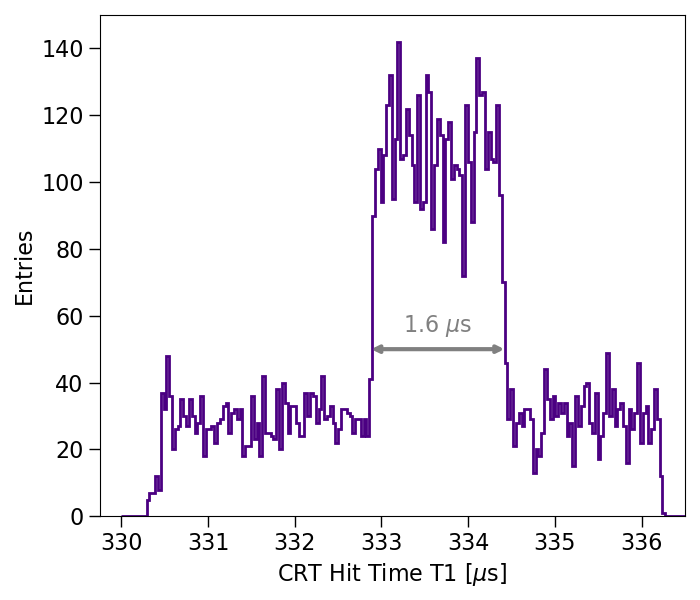
\includegraphics[width=\linewidth]{CRT_T1_TopHat}
\caption{CRT hit time T1}
\label{fig:topHat_T1}
\end{subfigure}%
\hfill
\begin{subfigure}[h]{0.495\linewidth}
\centering    
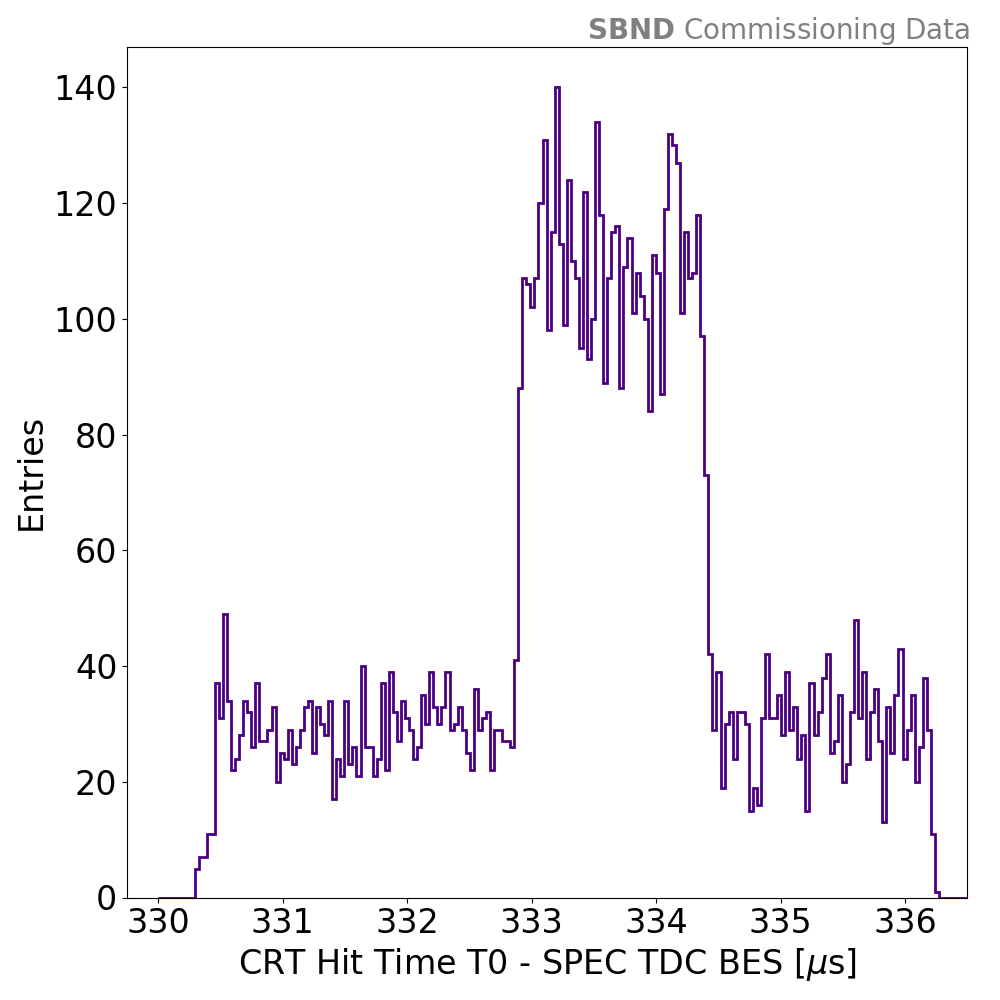
\includegraphics[width=\linewidth]{CRTT0_SPEC_TopHat}
\caption{CRT hit time T0}
\label{fig:topHat_T0}
\end{subfigure}
\caption[Reconstructed Beam Spill Using CRT Sharps]{
Beam spill reconstructed using (a) CRT hit time T1 and (b) CRT hit time T0 combined with the SPEC-TDC timing information. 
}
\label{fig:topHat}
\end{figure}


%The resolution of the T0 and T1 clock were shown earlier to be $\mathcal{O}$(2 ns), surpassing the requirement.
%Both methods are able to reconstruct the "top hat" shape of the beam spill and show good agreement with each other.
%Additionally, combining timestamps recorded by the SPEC-TDC with other hardware subsystems is a versatile tools for multiple purposes, from timing resolution characterisation to timing reconstruction.

The next step was to reconstruct the bucket structure of the BNB, made up of 81 buckets of Gaussian width 1.308 ns and separated by 19 ns.
Given the limited statistics of the sample to fully plot 81 buckets of a whole beam spill, the buckets were overlaid on top of each other by applying a modulus of 19 ns.
The resulting beam buckets using CRT hit time T1 and CRT hit time T0 combined with the SPEC-TDC timestamps are shown in Fig. \ref{fig:beamBucket_T1} and \ref{fig:beamBucket_T0} respectively.
Using the CRT hit time T1, the beam bucket was resolved even with the limited statistics, recovering a Gaussian width of 3.2 ns.
However, from the CRT hit time T0 distribution, the Gaussian bucket is more smeared out with a larger width of 3.5 ns. 
This is due to the resolution of the T0 clock being shown to be $\mathcal{O}$(2 ns), which is larger than the width of the beam bucket.

\begin{figure}[ht!]
\begin{subfigure}[h]{0.495\linewidth}
\centering    
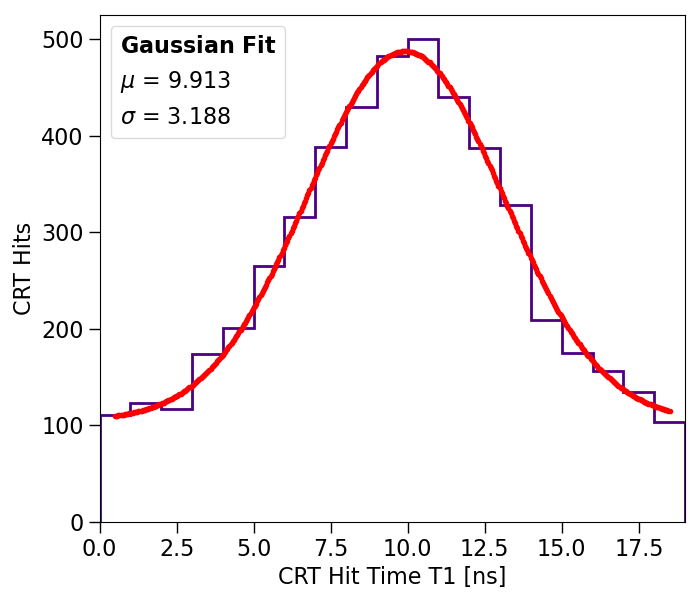
\includegraphics[width=\linewidth]{CRT_T1_Bucket}
\caption{CRT hit time T1}
\label{fig:beamBucket_T1}
\end{subfigure}%
\hfill
\begin{subfigure}[h]{0.495\linewidth}
\centering    
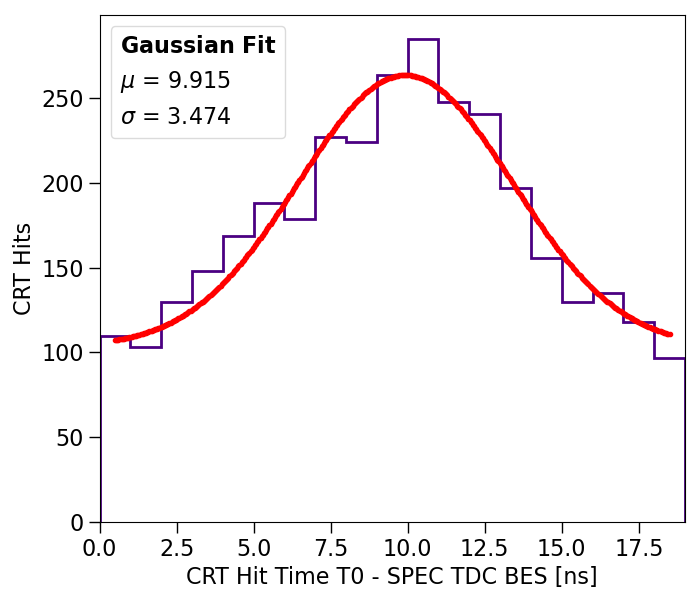
\includegraphics[width=\linewidth]{CRTT0_SPEC_Bucket}
\caption{CRT hit time T0}
\label{fig:beamBucket_T0}
\end{subfigure}
\caption[Reconstructed Beam Bucket Using CRT Sharps]{
Beam bucket reconstructed using (a) CRT hit time T1 and (b) CRT hit time T0 combined with the SPEC-TDC timing information. 
}
\label{fig:beamBucket}
\end{figure}

Both the reconstruction of the beam spill and beam bucket demonstrate that the CRT hit time T0 can be utilised together with the timing information recorded by the SPEC-TDC.
This alternative timing reconstruction shows promising early results and certainly has the potential for more improvements.
Additionally, this showcases the versatile usages of the SPEC-TDC, where its recorded timestamps can be used in conjunction with other detection subsystems. 

%********************************** %Third Section  **************************************
\section{Timing Performance of CAENV1730 Digitisers}
\label{sec4PMT}

The next focus is on the timing characterisation of PMT readout electronics, CAENV1730SB digitisers. 
Section \ref{subsec41PMT} provides a description of the CAENV1730's internal clocks.
An evaluation of the timing synchronisation across multiple digitisers is presented in Section \ref{subsec42PMT} and a clock jittering correction method is given in Section \ref{sec:jitter_correction}.

\subsection{Internal Clock and Timestamp Structure}
\label{subsec41PMT}

%clock of a single digitiser
%The clock distribution of the CAEN digitiser is made up of two clock domains in the hardware, OSC-CLK and REF-CLK \cite{caen1730}.
%The OSC-CLK is a fixed internal oscillator that has a frequency of 50 MHz. 
%This clock is responsible for handling communication between the motherboard and the mezzanines such as local bus, universal serial bus and optical link.

%The source of the REF-CLK can either be internal or external.
%For internal mode, the REF-CLK is referenced to the OSC-CLK of frequency 50 MHz.
%For external mode, the REF-CLK is fed by an external frequency via the CLK-IN connector. 

A description of the PMT readout electronics, CAENV1730SB digitisers, is summarised in Section \ref{sec:readout}.
The internal clock of interest is called REF-CLOCK in the clock domains of a CAEN digitiser \cite{caen1730}.
The REF-CLK is a clock chain responsible for a synchronous sampling and triggering rate, and thus, the timing precision of the CAEN digitiser.
Its frequency serves as an input to a clock distribution device AD9510, generating three clock types: (1) an ADC sampling clock, (2) a trigger clock and (3) an output clock for external use.
The AD9510 device must be programmed for the input REF-CLK frequency so that all three clocks are in phase with the input and with each other.

%What are the clocks
The ADC sampling clock has a frequency of 500 MHz to enabled the waveform sampling with the tick value of 2 ns/tick. 
The trigger clock operates at 125 MHz with a tick value of 8 ns/tick, and is responsible for handling the triggering and synchronisation logic.
However, since it is read every two clock cycles, it potentially has a fluctuation of up to 16 ns/tick.
The last clock is a programmable frequency output via the CLK-OUT connector and can be propagated to another CAEN digitiser for synchronisation purposes.

%What are input to the clocks
At SBND, CAEN digitisers are configured to use an external clock input to the REF-CLK with signals from the WR timing system described in Section \ref{subsec41TimeRef}.
The external clock is input via the CLK-IN connector of the digitiser, with frequency depending on the clock synchronisation scheme.
This signal behaves as a \textit{metronome frequency} for all three clocks described above.
Additionally, the PPS signal is input to the S-IN connector of the digitiser and is used by the trigger clock.
It resets the counter of the trigger clock every second so that the timestamps output by CAEN digitisers share the \textit{same reference frame} with respect to the whole second as other readout electronics.

\begin{figure}[b!] 
\centering    
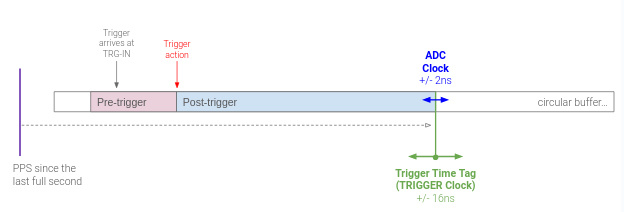
\includegraphics[width=1.0\textwidth]{TTT_diagram}
\caption[Timing Structure of a Waveform Digitised by CAEN]{
Timing structure of a waveform digitised by CAEN digitisers.
}

\label{fig:TTTDiagram}
\end{figure}

%It can be either from the SVEC-FD modules, which make the standard 10 MHz clock, or can be from another CAEN digitiser CLK-OUT, which make the standard 62.5 MHz frequency.

%CAEN Timestamp
Unlike the timestamp generated by FEB modules or the SPEC-TDC, where it is the number of clock ticks upon receiving a signal, the timestamp produced by CAEN digitisers is structured differently.
Fig. \ref{fig:TTTDiagram} illustrates the time structure of a waveform recorded by CAEN digitisers.
Upon receiving a trigger at the TRG-IN connector, as shown in grey, there is a latency before the digitiser acting on the trigger, as shown in red.
The waveform length can be any portion pre- or post-trigger as shown by the red and blue boxes.
For every trigger, the CAEN trigger clock produces a timing object called a trigger time tag.
However, the trigger time tag is not instantaneous upon the trigger arrival, it is instead the timestamp value of the last tick on the waveform, as shown in green.
Therefore, a careful timing reconstruction is needed when decoding the waveforms.

%to ensure consistency in comparing the timestamps of the CAEN digitiser and the SPEC-TDC, they need to be corrected to the same reference frame, which was chosen to be the time at which the trigger leaves the PTB front face.
%The TTT is the number of ticks (8 ns/tick) since the trigger clock last receives a PPS signal.
%Meanwhile, the CAEN digitiser generates a timestamp object called TTT associated with every trigger, and this timestamp is not , as illustrated in Fig. \ref{fig:TTTDiagram}. 
%If both the CAEN digitisers and the SPEC-TDC synchronised with each other, the difference in the timestamps should be 0.
%The timestamp embedded in the Trigger Time Tag accounts for a fixed buffer time the digitiser takes to generate the Trigger Time Tag upon receiving a trigger.
%This timestamp also points the end the recorded waveform.

\subsection{Evaluation of Clock Synchronisation}
\label{subsec42PMT}

%clock synchronisation
Multiple CAEN digitisers can be synchronised to behave as if a single digitiser.
It is crucially important to record PMT waveforms in synchronisation since they are the key ingredients for timing reconstruction with a resolution $\mathcal{O}$(2 ns) as previously detailed in Sec \ref{sec:reco_pds}.
The synchronisation can be achieved through two different clock synchronisation schemes: (1) fan out and (b) daisy chain, as shown in Fig. \ref{fig:clockScheme_fanout} and \ref{fig:clockScheme_daisy} respectively.

\begin{figure}[b!]
\begin{subfigure}[h]{0.495\linewidth}
\centering    
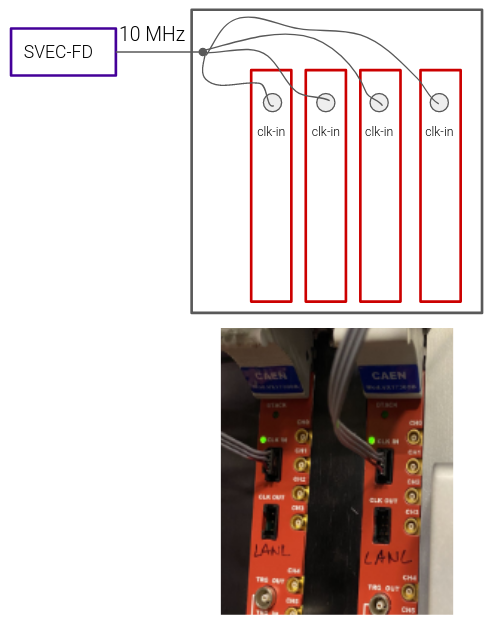
\includegraphics[width=\linewidth]{fanout}
\caption{Fan out}
\label{fig:clockScheme_fanout}
\end{subfigure}%
\hfill
\begin{subfigure}[h]{0.495\linewidth}
\centering    
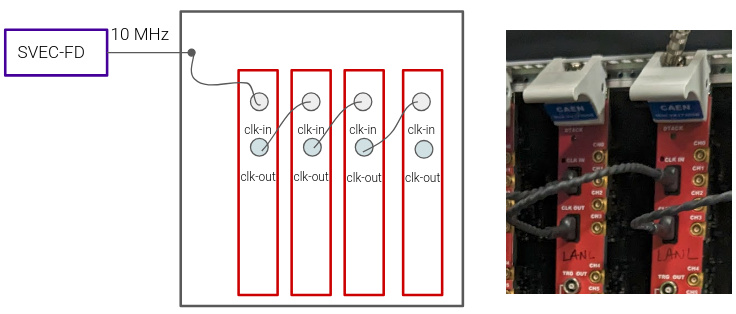
\includegraphics[width=\linewidth]{daisychain}
\caption{Daisy chain}
\label{fig:clockScheme_daisy}
\end{subfigure}
\caption[Clock Synchronisation Schemes]{
Diagram illustrating two clock synchronisation schemes for CAENV1730SB digitisers, (a) fan out and (b) daisy chain.
}
\label{fig:clockScheme}
\end{figure}

In fan out mode, each digitiser is input with the clock signal set at 10 MHz clock.
The 10 MHz was chosen at the time since it is the highest frequency produced by the SVEC-FD module.
The clock signal is distributed to a fan out module, and then into the CLK-IN connector of each digitiser.
The cable length of each clock signal is identical so that all clock signals arrive at CAEN digitisers at the same time.

%The 10 MHz clock is produced by the SVEC-FD card, input to an LVDS fan out, and then into the CLK-IN connector of each digitiser.
%In this configuration, every CAEN digitiser should receive identical external frequency for the REF-CLK that generates the sampling and trigger clock.

In daisy chain mode, the first CAEN digitiser in the daisy chain receives the 10 MHz clock, referred to as the master clock.
Its clock is then propagated to the next digitiser in the chain, referred to as the slave clock.
The master clock can be precisely programmed with a delay $\mathcal{O}$ (300 ps) to account for cable lengths, ensuring that the master and slave clocks are in phase with each other.
The clock propagation continues from one digitiser to the next digitiser in the chain, until the last digitiser in the chain is in the same clock phase as the first one.  

%set up
%Over the summer of 2023, the author has travelled to Fermilab for the second time to conduct the work on evaluating the timing resolution and synchronisation of the CAEN digitisers.
%The goal was to achieve synchronisation across all 8 CAEN digitisers and with respect the timing system of the DAQ.

The timing characterisation study was carried out to determine which clock synchronisation scheme provides the best precision and stability. 
The setup consisted of 8 CAEN digitisers located in the same crate. 
Each digitiser received an identical trigger with the same cable length so every digitiser was triggered simultaneously.
The trigger rate was set as 1 Hz for simplicity.

To evaluate the synchronisation of CAEN digitisers, their timestamps of triggered events were directly compared against the same timestamps recorded by the SPEC-TDC since both are referenced to the 
PPS signal.
Similar to the approach with the CRT readout electronics, the SPEC-TDC offers a higher level of precision compared to the CAEN digitiser, 700 ps compared to $\mathcal{O}$(2 ns). 
For an ideal synchronisation, the timestamps of every triggered event from every digitiser should be identical with respect to each other, and also with respect to the SPEC-TDC after cable correction.

%The trigger signal was also input to the SPEC-TDC for timestamping.
%Timestamps of the trigger recorded by the CAEN digitisers and the SPEC-TDC can be compared against each other .
%Therefore, the comparison helps characterising the resolution of the timestamps produced the CAEN digitiser. 
%This comparison also evaluates whether each CAEN digitiser is synchronised with respect to the PPS signal.

%Result from daisy chain
%The daisy chain clock scheme underwent testing across multiple DAQ runs over a few days. 

Some results of synchronisation using the daisy chain are shown in Fig. \ref{fig:daisychainSPEC}, depicting the differences of timestamps CAEN digitisers from the SPEC-TDC as a function of the event 
number.
Only 4 out of 8 CAEN digitisers are shown for run 7980 and run 8060, however, similar results were observed for the rest of the digitisers.
Run 7980 in Fig. \ref{fig:run7980} demonstrates a perfect synchronisation across all 8 CAEN digitisers.
Their differences with respect to the SPEC-TDC are constant at 0 across all the events and all the digitisers.
This shows a very good and stable synchronisation.

In contrast, run 8060 exhibited some interesting effects as shown in Fig. \ref{fig:run8060}.
Firstly, board 5 shows a straddling effect, where the observed differences jitters between 0 and 8 ns.
This behaviour could be due to the CAEN trigger clock of the CAEN digitiser being read out every 2 clock cycles, introducing some fluctuations.
Moreover, board 7, which received a clock signal from board 5 in the daisy chain, drifted by 8 ns.
Following that, board 9, receiving clock from board 7, also drifted by 8 ns. 
This demonstrates that if one clock in the daisy chain drifts, subsequently clocks in the chain also drift.

\begin{figure}[htbp!]
\begin{subfigure}[h]{1.00\linewidth}
\centering    
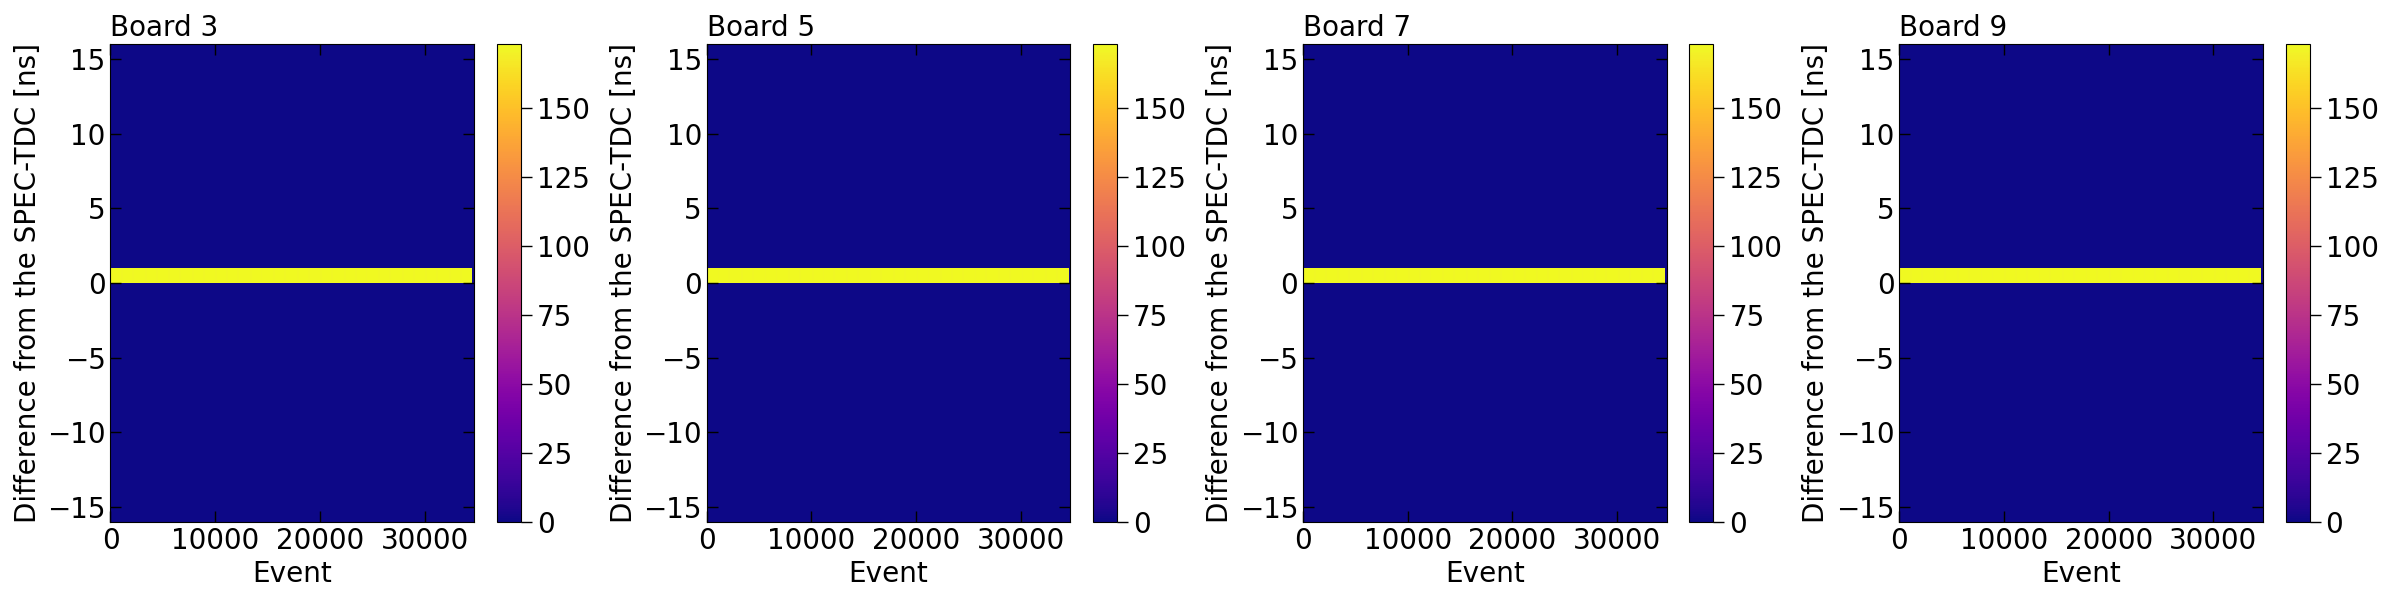
\includegraphics[width=\linewidth]{TTT_SPEC_diff_run7980}
\caption{Run 7980}
\label{fig:run7980}
\end{subfigure}
%\vspace{0.5cm}
\begin{subfigure}[h]{1.00\linewidth}
\centering    
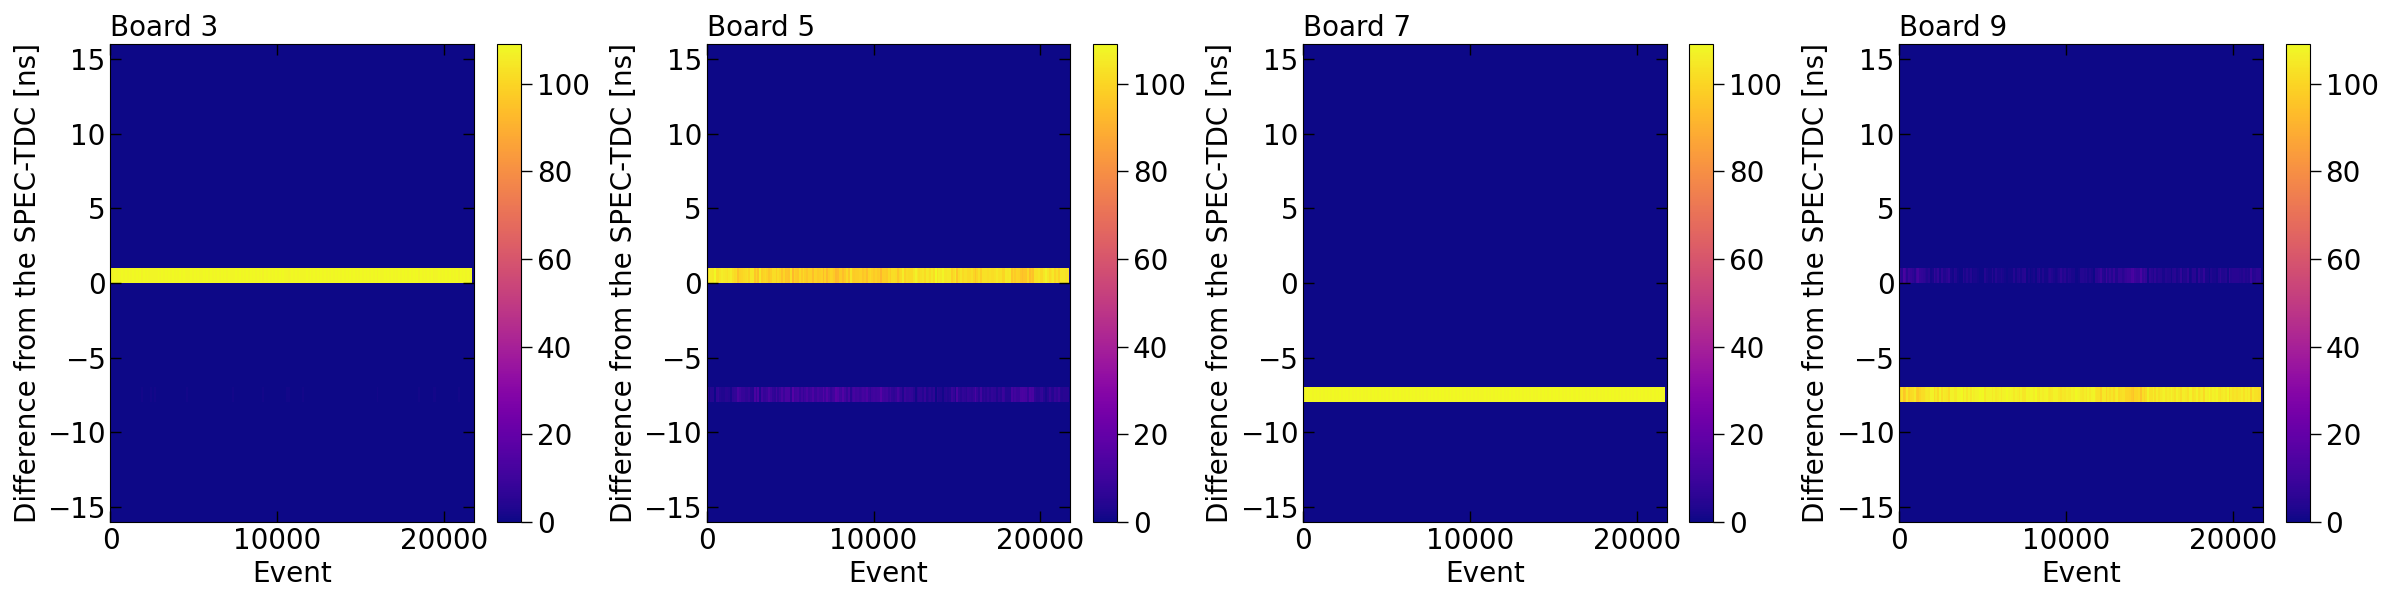
\includegraphics[width=\linewidth]{TTT_SPEC_diff_run8060}
\caption{Run 8060}
\label{fig:run8060}
\end{subfigure}%
\caption[Variation of CAEN Timestamps Using the Daisy Chain Clock Scheme]{
Differences in trigger timestamps between CAEN digitisers and the SPEC-TDC with the CAEN digitisers using the daisy chain clock scheme.
}
\label{fig:daisychainSPEC}
%\end{figure}
\vspace{0.5cm}
%\begin{figure}[h!]
\begin{subfigure}[h]{1.00\linewidth}
\centering    
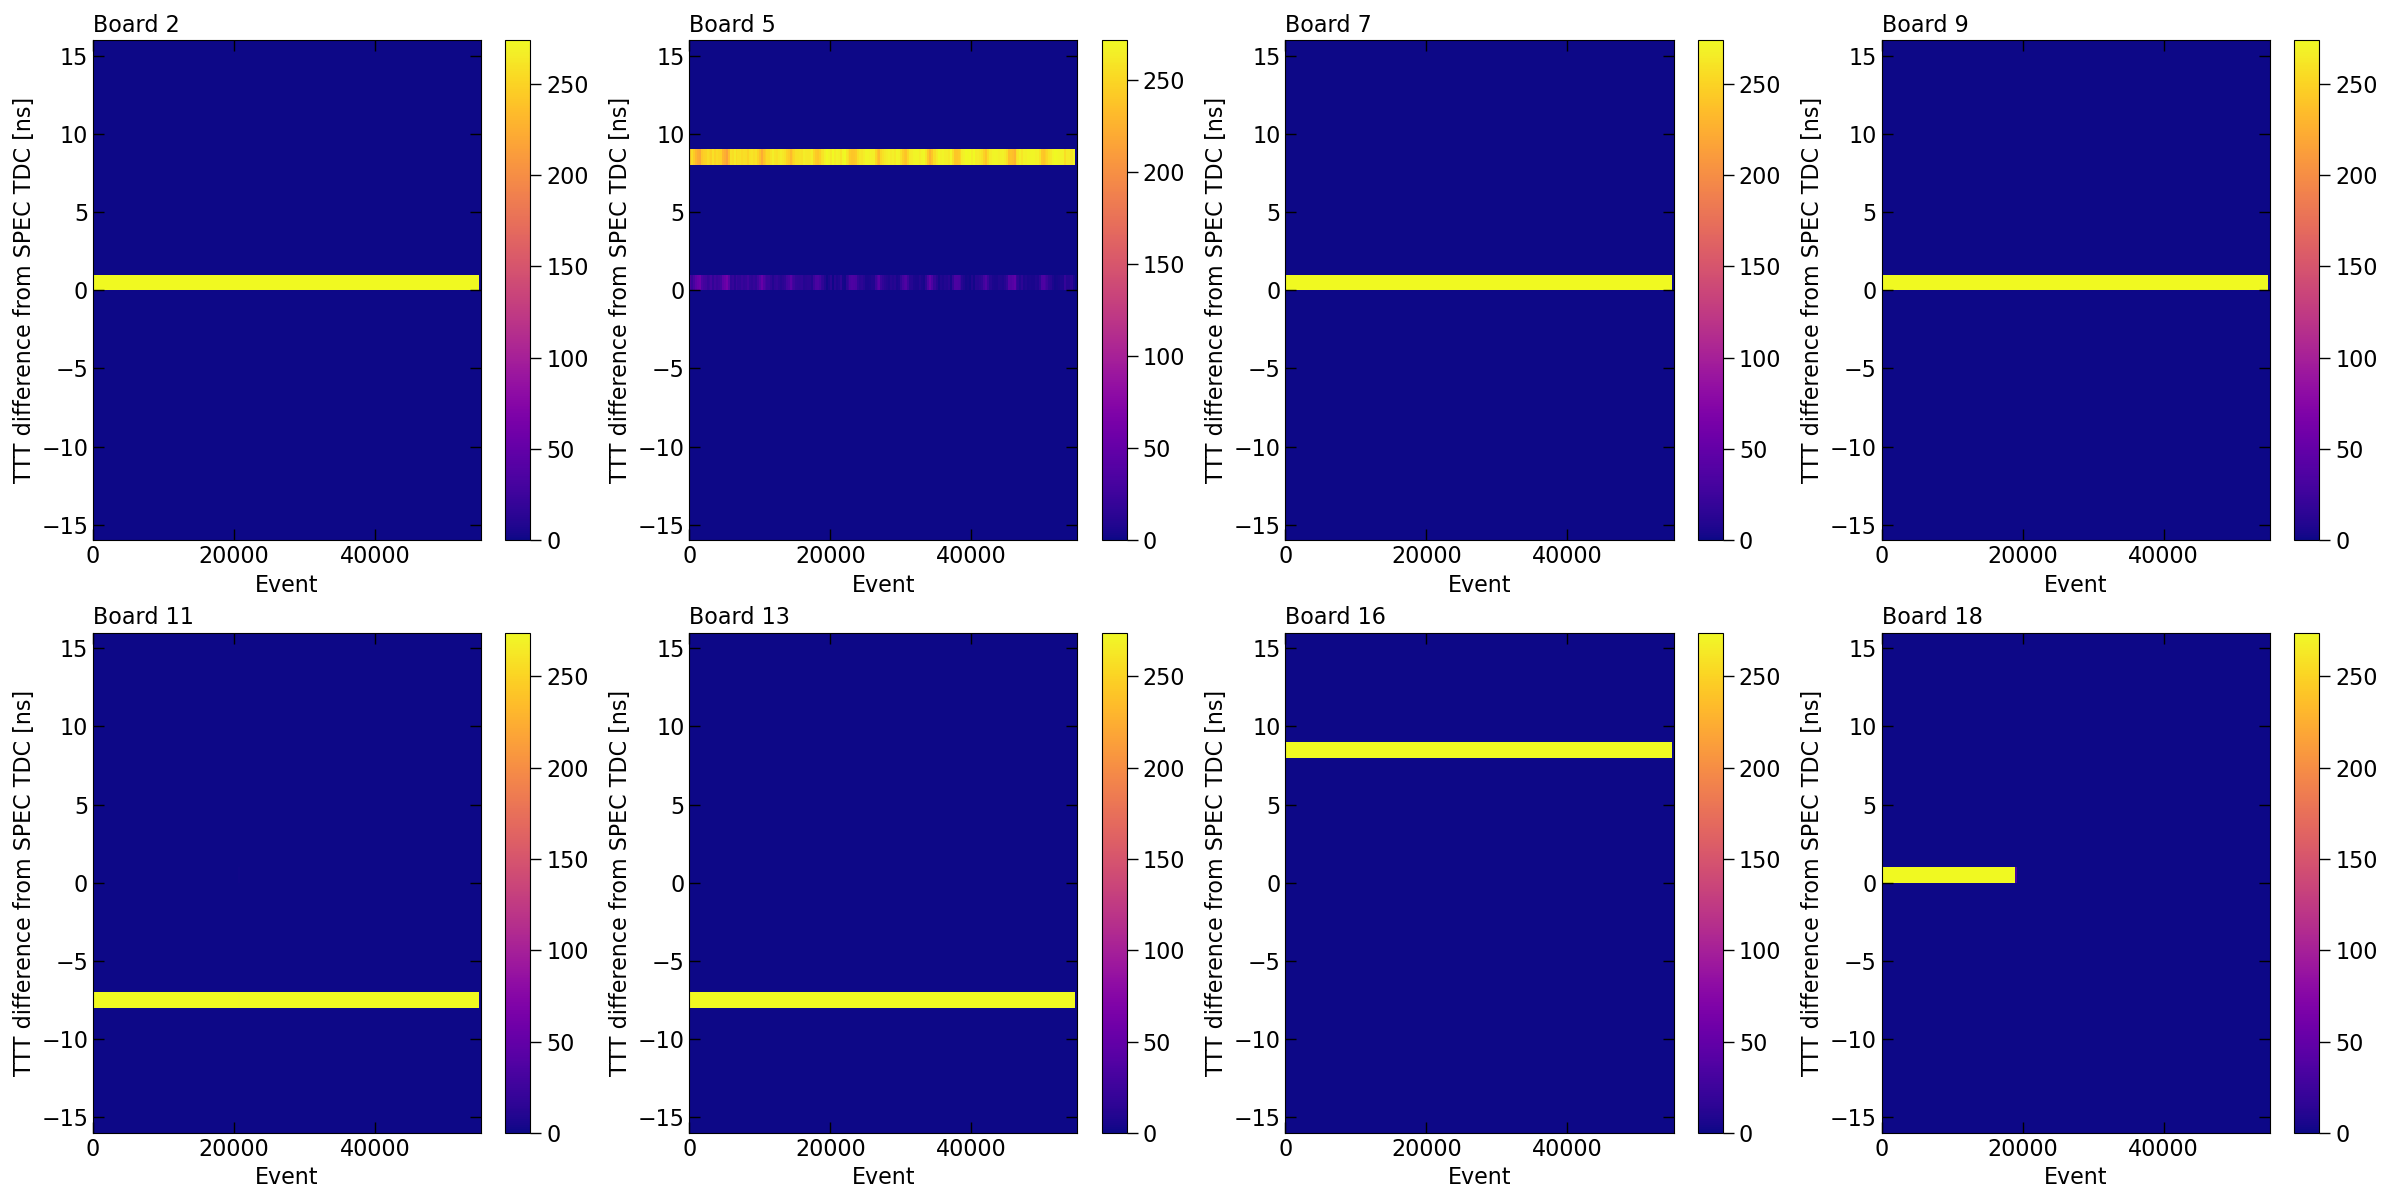
\includegraphics[width=\linewidth]{TTT_SPEC_diff_run8178}
\caption{Run 8178}
\end{subfigure}
%\vspace{0.5cm}
\begin{subfigure}[h]{1.00\linewidth}
\centering    
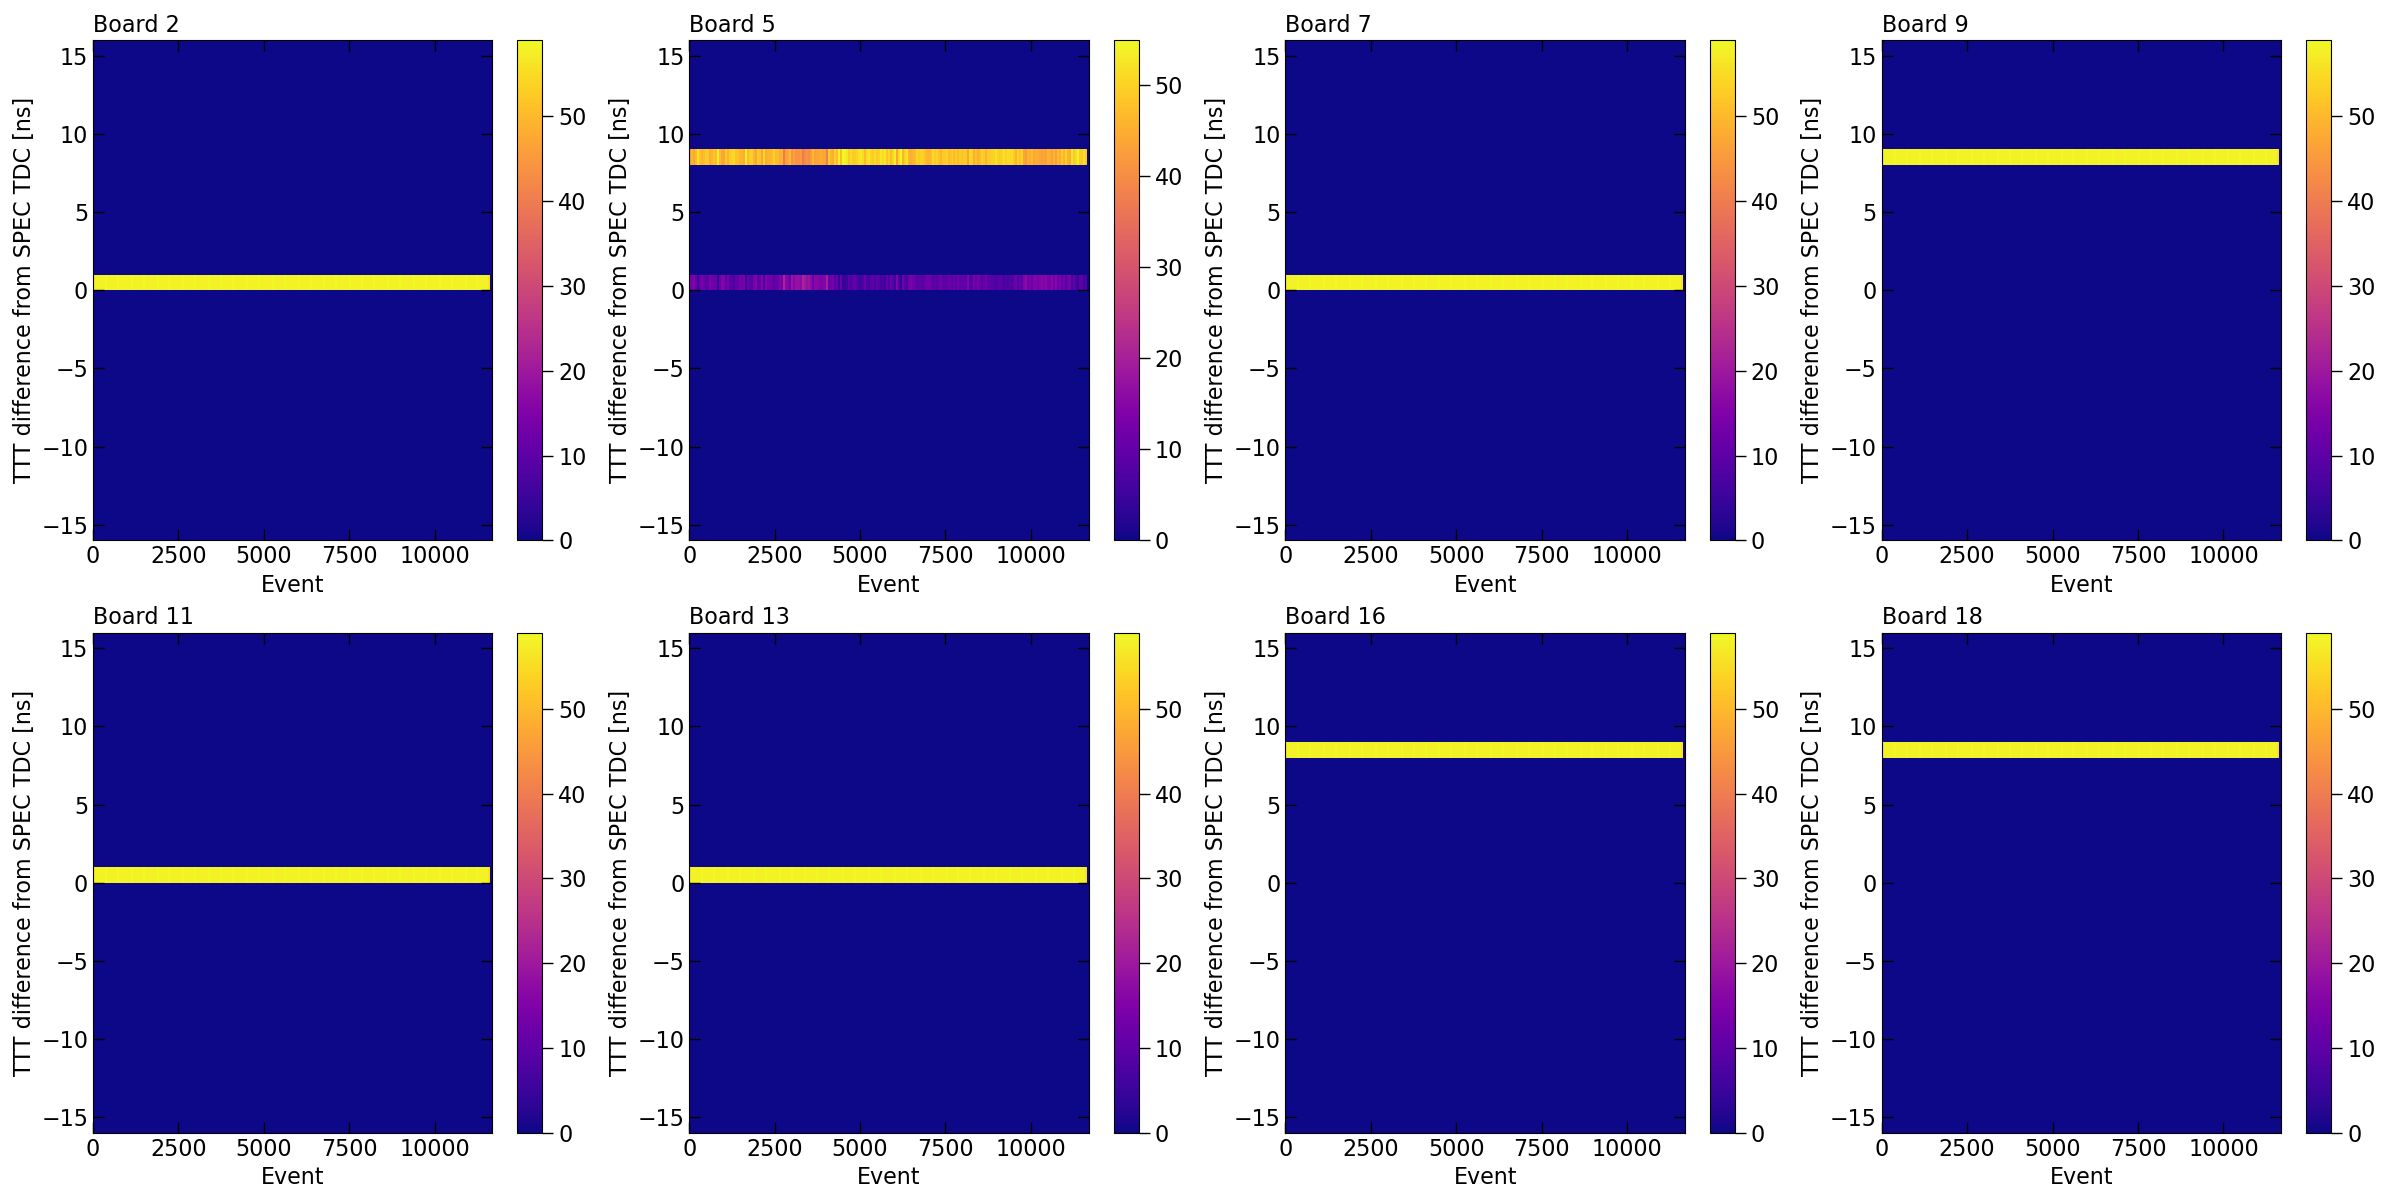
\includegraphics[width=\linewidth]{TTT_SPEC_diff_run8196}
\caption{Run 8196}
\end{subfigure}%
\caption[Variation of CAEN Timestamps Using the Fan Out Clock Scheme]{
Differences in trigger timestamps between CAEN digitisers and the SPEC-TDC with the CAEN digitisers using the fan out clock scheme.
}
\label{fig:fanoutSPEC}
\end{figure}

The same test was repeated for the fan out scheme. % where multiple DAQ runs were conducted over a few days.
Some example results are shown in Fig. \ref{fig:fanoutSPEC} for run 8178 and run 8196.
Firstly, in both of these runs, board 5 shows the same straddling effect, causing its timestamps to jitter by 8 ns.
The second observation is that the timestamp differences vary randomly between digitisers and across different runs. 
For instance, the timestamp difference of board 9 is stable at -8 ns in run 8178 but stays at +8 ns in run 8196.

This behaviour is due to the input frequency to the CLK-IN connector set at 10 MHz.
As previously explained, the trigger clock is generated by the AD9510 device, which must be in phase with the input frequency. 
However, the trigger clock operates at a frequency of 125 MHz, while the input frequency is at 10 MHz. 
Since these frequencies are not multiples of each other, they cannot be in phase.
To generate an out-of-phase frequency, the AD9510 device latches onto the first rising edge of the input frequency upon the digitiser initialisation.
This results in a random phase offset at the beginning of every run, causing the timestamps to vary from run to run and from board to board. 

%settle for daisy chain over fan
Comparing the two clock schemes, the daisy chain mode offers a better synchronisation across the 8 CAEN digitisers compared to the fan out mode.
In the daisy chain scheme, only the first digitiser in the daisy chain receives the external 10 MHz clock.
The master clock will have a random phase offset that is propagated down the daisy chain, resulting in synchronisation across all digitisers.
However, the clock drift effect was observed during the testing of the daisy chain scheme and therefore, a correction is necessary.

\subsection{Clock Jittering Correction}
\label{sec:jitter_correction}

%setup
To further characterise the timing of the CAEN digitiser, another study was carried out to verify if all 8 CAEN digitisers can digitise waveform in synchronisation with each other within 1 ns. 
The same setup was used as described in the previous section, with a new addition of digitising the waveform of the trigger signal in channel 15 of every digitiser.
All cable lengths were identical so that all trigger signals took the same amount to propagate to the digitisers.
The daisy chain clock scheme was also calibrated so that the clock propagation from the master clock to the slave clock was delayed by a precise amount so that their clocks were exactly in phase.
This was to ensure that trigger signals were simultaneously timestamped and digitised.

Examples of digitised waveforms of trigger signals are plotted in Fig. \ref{fig:full_wfm} for four digitisers, where trigger signals can be seen as a single square wave per digitiser.
To examine if trigger signals were digitised simultaneously, zooming into the rising edges of trigger signals is plotted in Fig. \ref{fig:zoom_edge}.
Board 3, 5 and 9 are in synchronisation except for board 7.
The rising edge of board 7 is at a different location compared to other boards, showing that its clock jittered.
This behaviour although did not occur frequently, it was unpredictable and could appear across different events, different runs and different boards. 
Therefore, a jittering correction was derived to account for clock jittering scenarios.

\begin{figure}[ht!]
\begin{subfigure}[h]{1.00\linewidth}
\centering    
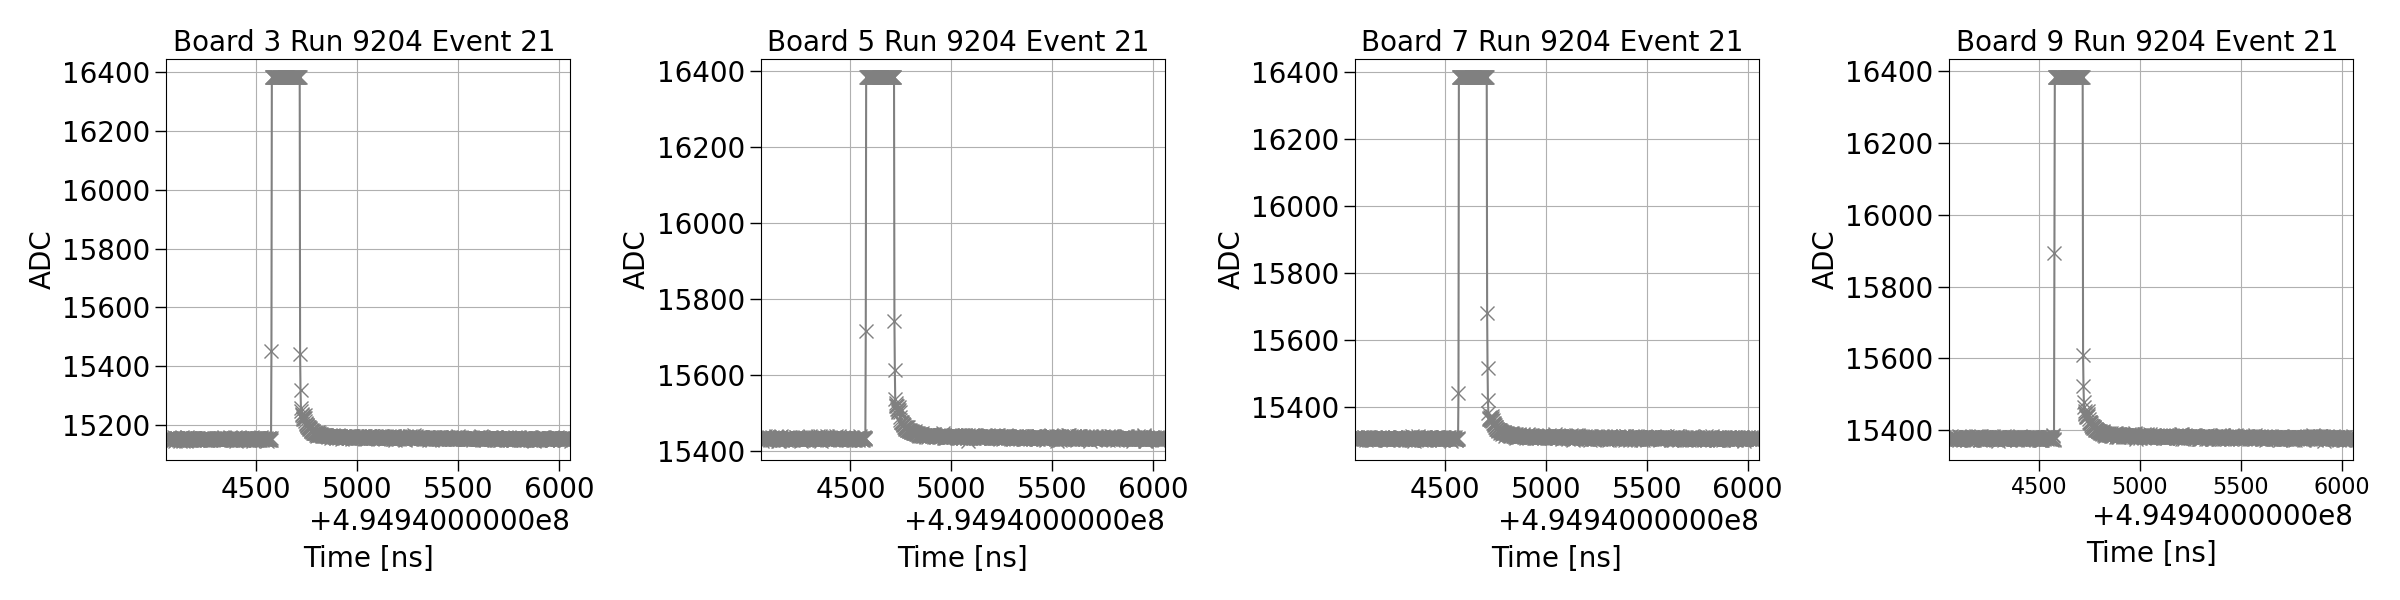
\includegraphics[width=\linewidth]{jitter_before_unzoom}
\caption{Full waveforms}
\label{fig:full_wfm}
\end{subfigure}
\vspace{0.5cm}
\begin{subfigure}[h]{1.00\linewidth}
\centering    
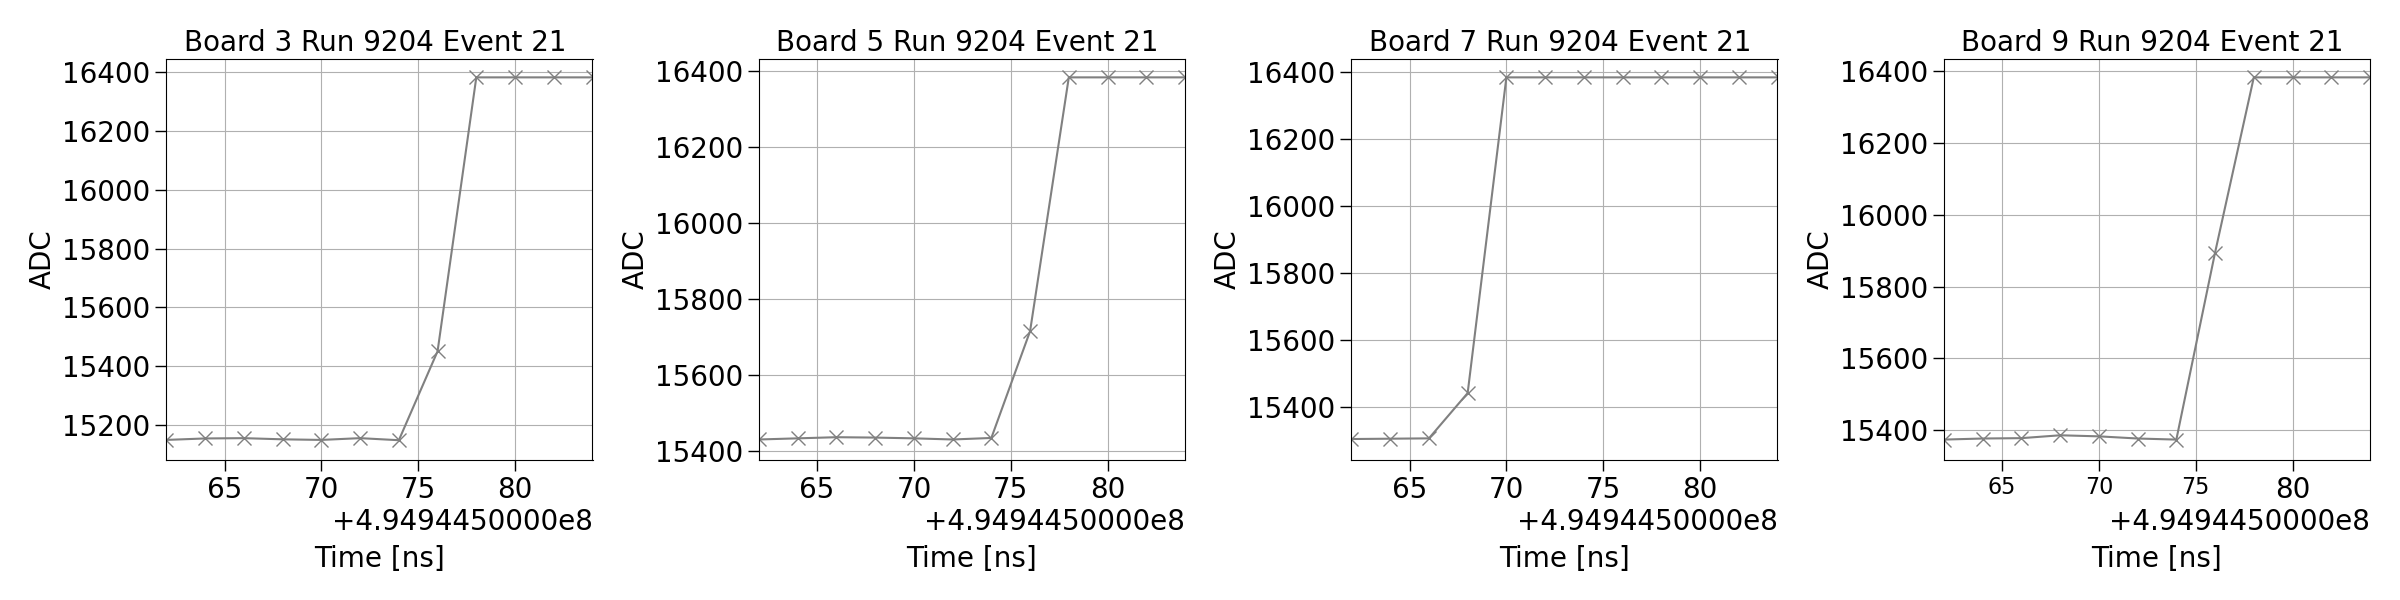
\includegraphics[width=\linewidth]{jitter_before_zoom}
\caption{Zoom into the rising edge}
\label{fig:zoom_edge}
\end{subfigure}%

\caption[Digisted Waveforms of Trigger Signals]{
Digitised waveforms trigger signals, including (a) full waveforms and (b) zoom into the rising edge.
}
\label{fig:trig_wfm}
\end{figure}

The timestamp of the rising edge of trigger signals digitised by CAEN digitisers was compared against the timestamp recorded by the SPEC-TDC of the same trigger signal.
This comparison helps the understanding of the clock jittering behaviour of the CAEN digitiser. 
Three identified cases of jittering are illustrated in Fig. \ref{subfig:jitter_before}.
The trigger waveform is plotted in grey, the rising edge is marked with a red cross and the timestamp of the trigger signal recorded by the SPEC-TDC is plotted as the vertical green line.

In the far left plot, the timestamp of the rising edge and the SPEC-TDC agree with each other and hence, the red cross and the green line align.
The middle left plot shows the first case of clock jittering of one whole sampling tick, equivalent to 2 ns.
This is due to the ADC sampling clock jitters while the triggering clock remains stable, resulting in a different tick value of the rising edge.
In the second case, the opposite situation arises such that the tick value of the rising edge timestamp is stable however the trigger clock jitters in the step of 8 ns.
This is illustrated in the middle right plot, where the rising edge and the SPEC-TDC differ by exactly 8 ns. 
The last case is the combination of jittering from both sampling and trigger clocks.
This is shown in the far right plot, where the difference between the rising edge and the SPEC-TDC is equal to the sum of the trigger and ADC sampling clock tick, totalling at 10 ns.

\begin{figure}[t!]
\begin{subfigure}[h]{1.00\linewidth}
\centering    
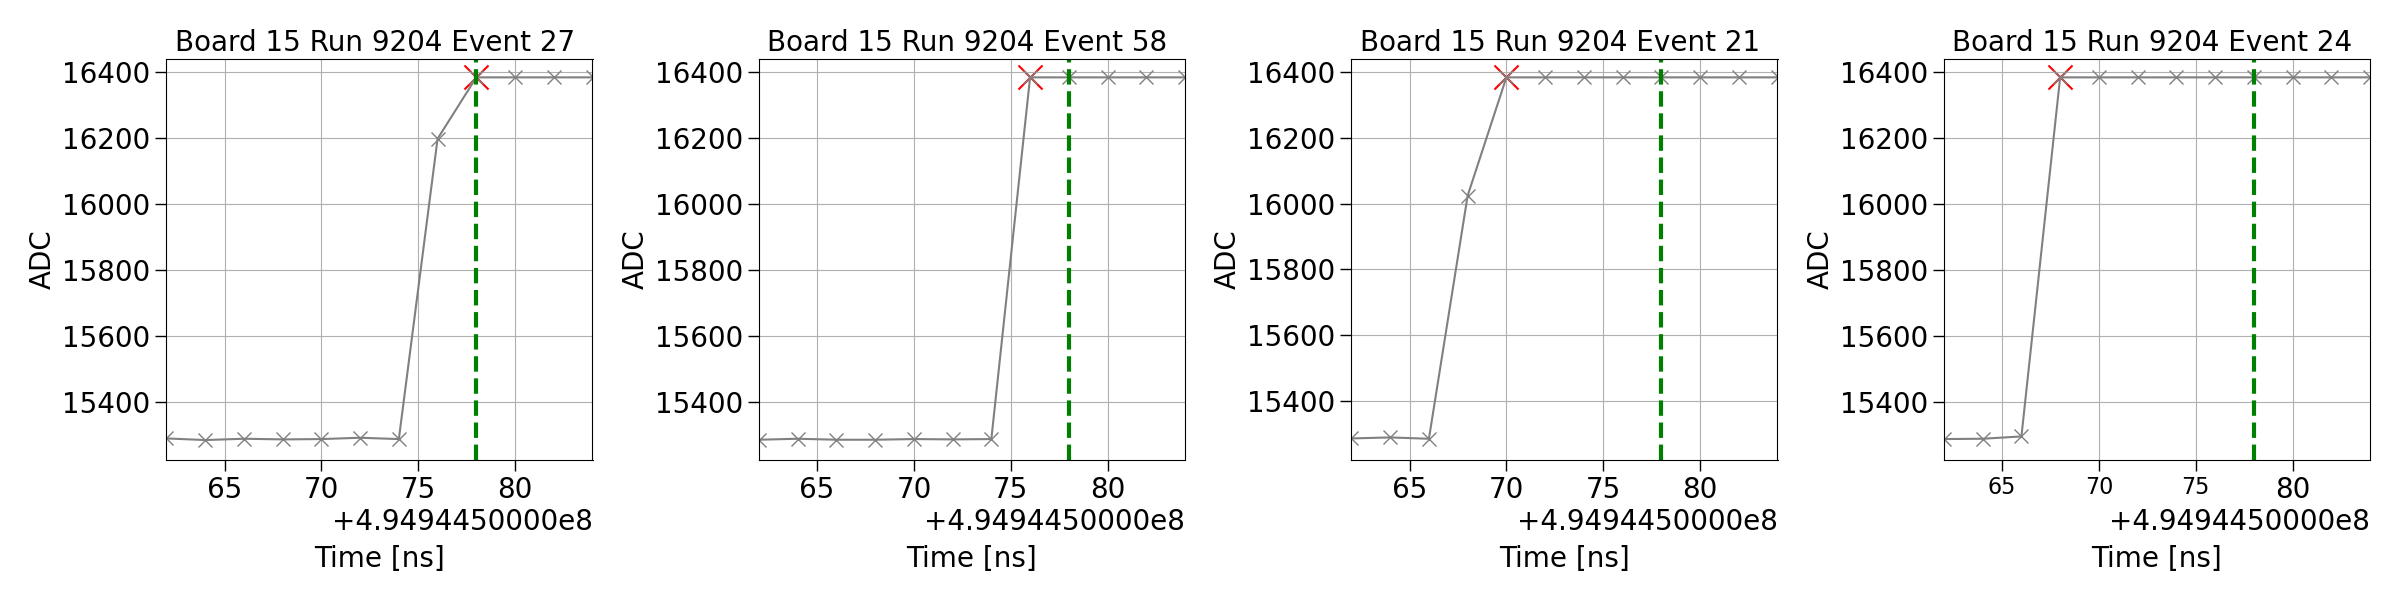
\includegraphics[width=\linewidth]{jitter_before}
\caption{Before Correction}
\label{subfig:jitter_before}
\end{subfigure}
\vspace{0.5cm}
\begin{subfigure}[h]{1.00\linewidth}
\centering    
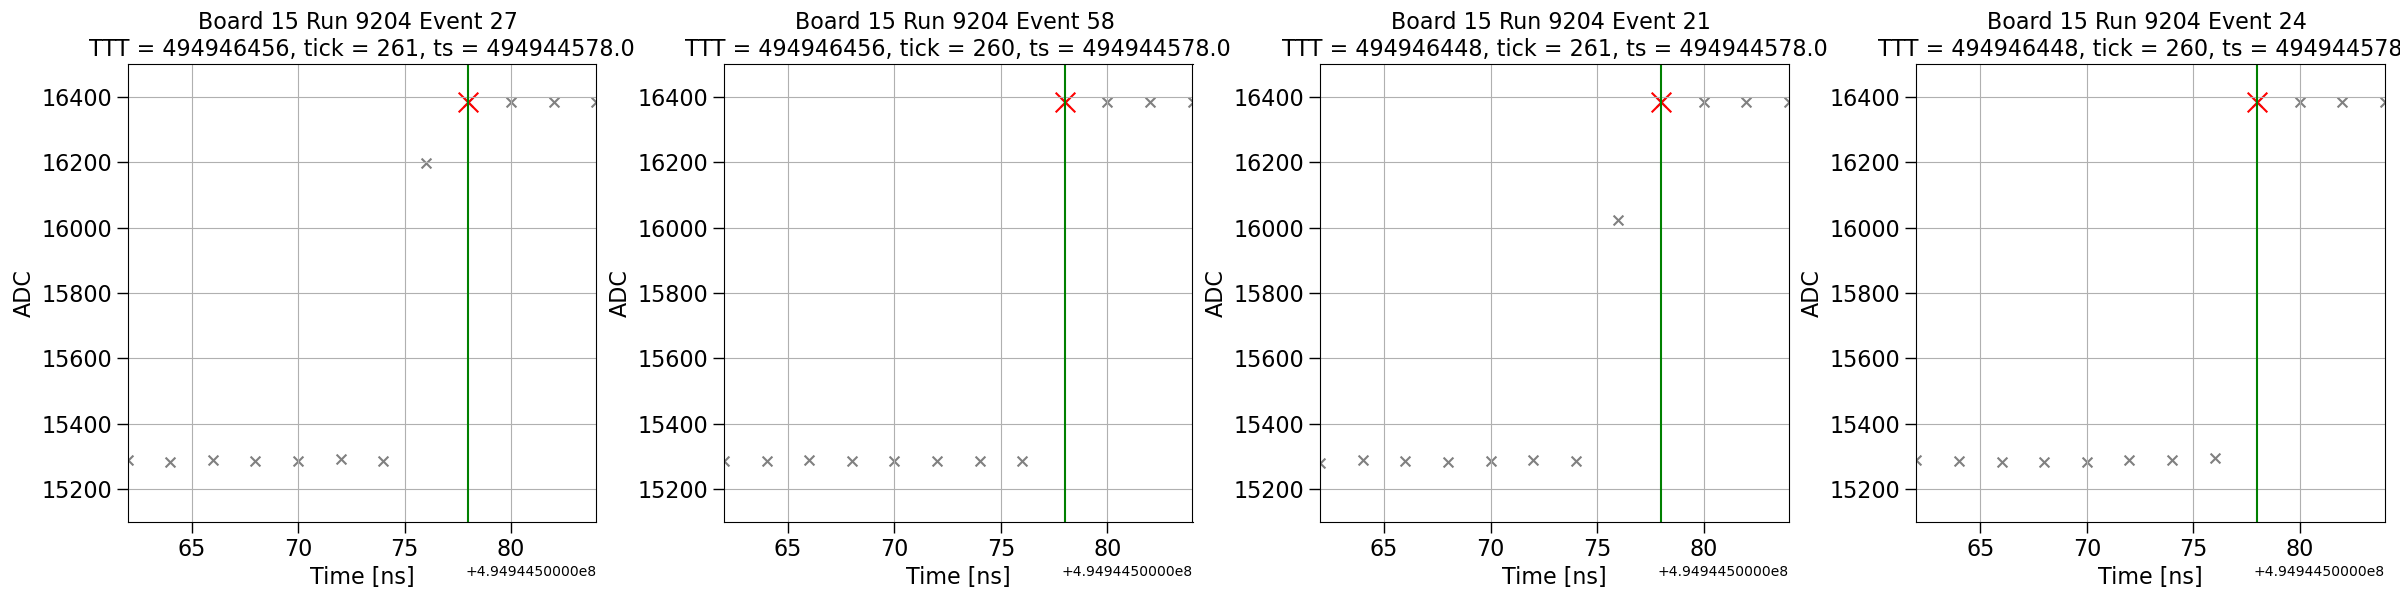
\includegraphics[width=\linewidth]{jitter_after}
\caption{After Correction}
\label{subfig:jitter_after}
\end{subfigure}%

\caption[Clock Jittering Correction Performed on Trigger Waveforms]{
Digitised waveforms of trigger signals zoom into the rising edge (a) before correction and (b) after correction.
}
\label{fig:jitterCorr}
\end{figure}

%how to correct for jittering:
This comparison exercise also demonstrated a possible clock jittering correction.
By digitising the trigger signal simultaneously on every digitiser, the recorded waveform of the trigger in combination with the SPEC-TDC provide all the necessary information to apply a correction.
One can simply derive the correction amount by performing the comparison as above.
The digitised trigger waveforms after applying correction are illustrated in Fig. \ref{subfig:jitter_after}, showing all the waveforms perfectly aligned to each other.

%Once this correction is applied to all events within the same run, one can also correct for the random clock phase initialisation across multiple runs within the same CAEN digitiser.
%This order of correction results in the perfect synchronisation across all events and all runs from different periods of time.
%For demonstration, this correction workflow was applied to the distribution of the tick-derived timestamp previously shown in Fig. \ref{subfig:Tickts_spec}.
%The correction was applied event by event followed by correction run by run as shown in Fig. \ref{fig:Tickts_spec_corr}, resulting in synchronisation across all the CAEN digitisers and also with respect to the PPS signal.

This correction method was validated using multiple runs over one month.
Each run duration varied from less than 1 hour up to more than 10 hours.
Fig. \ref{subfig:Tickts_spec_Nocorr} demonstrated the results conducted on a dataset of 30 runs, showing the 1D histogram of the difference between the timestamp of the rising edge as compared to the
 SPEC-TDC.
The plots are area normalised to directly compare across different run durations.
Before correction, some amount of jittering can be seen across different digitisers, events and runs, with peaks at 4 and 8 ns.
The correction was first applied event by event, as shown in Fig. \ref{subfig:Tickts_spec_corrEbyE}.
Then, the correction was applied run by run, as shown in Fig. \ref{subfig:Tickts_spec_corrRbyR}.
The result is a perfect alignment between the CAEN digitisers and the SPEC-TDC, with their differences forming a single peak at 0 ns.

\begin{figure}[ht!]

\begin{subfigure}[h]{1.00\linewidth}
\centering    
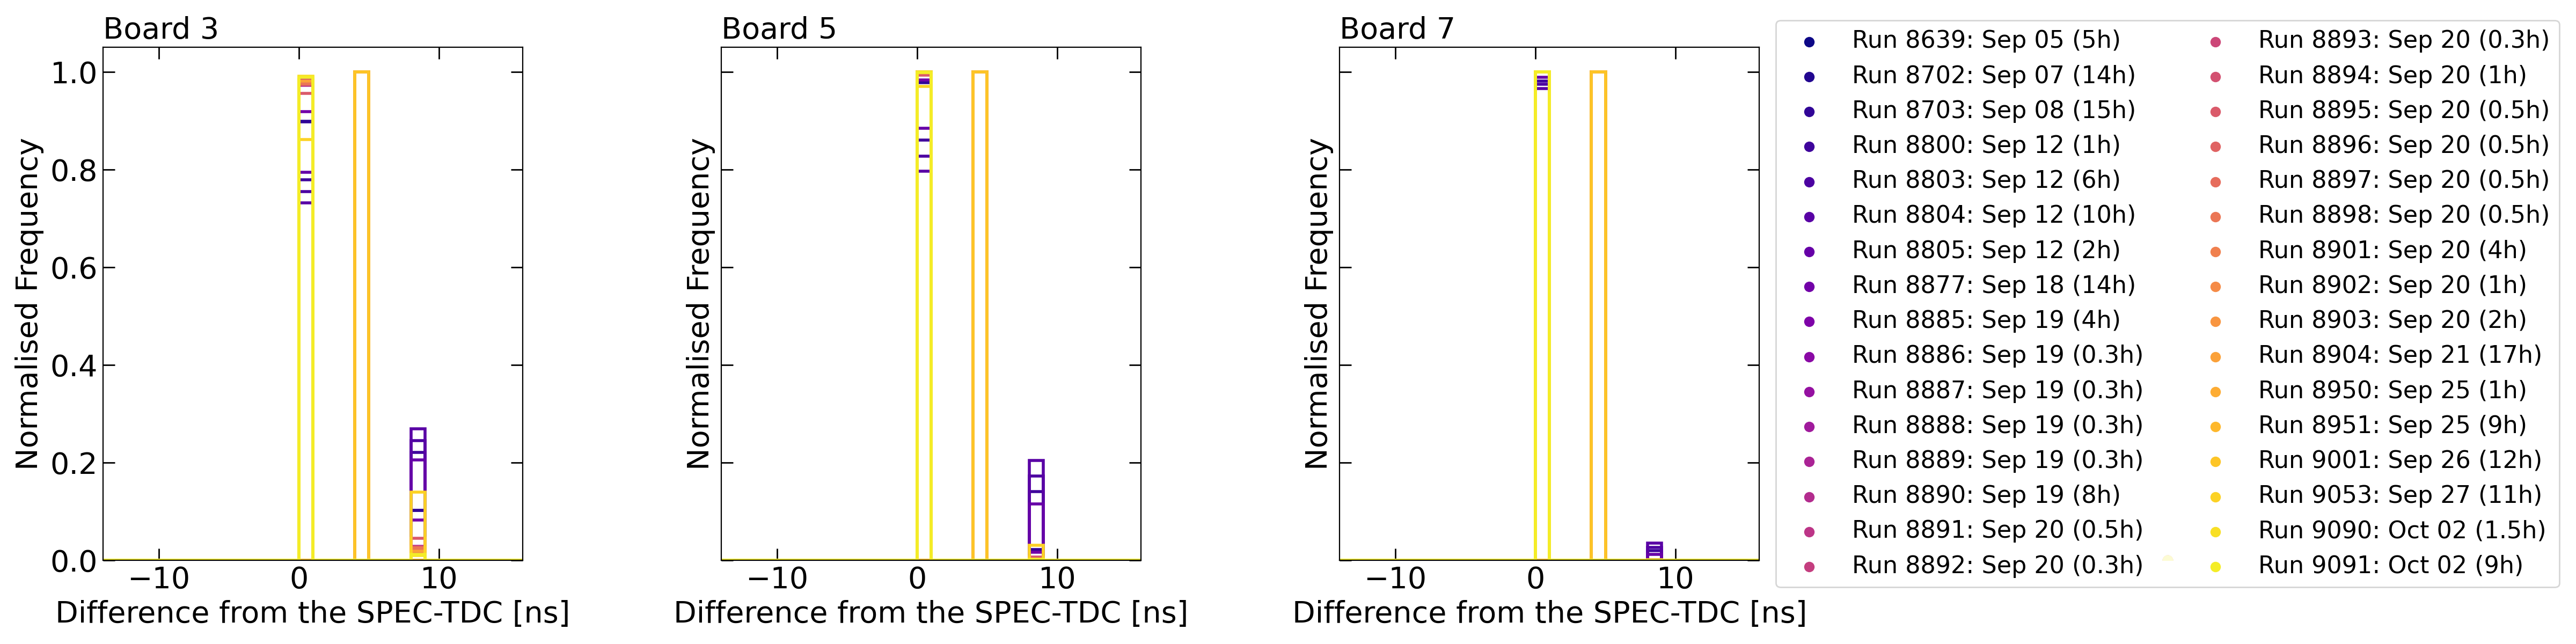
\includegraphics[width=\linewidth]{Tickts_spec}
\caption{Before correction}
\label{subfig:Tickts_spec_Nocorr}
\end{subfigure}
\vspace{0.5cm}
\begin{subfigure}[h]{1.00\linewidth}
\centering    
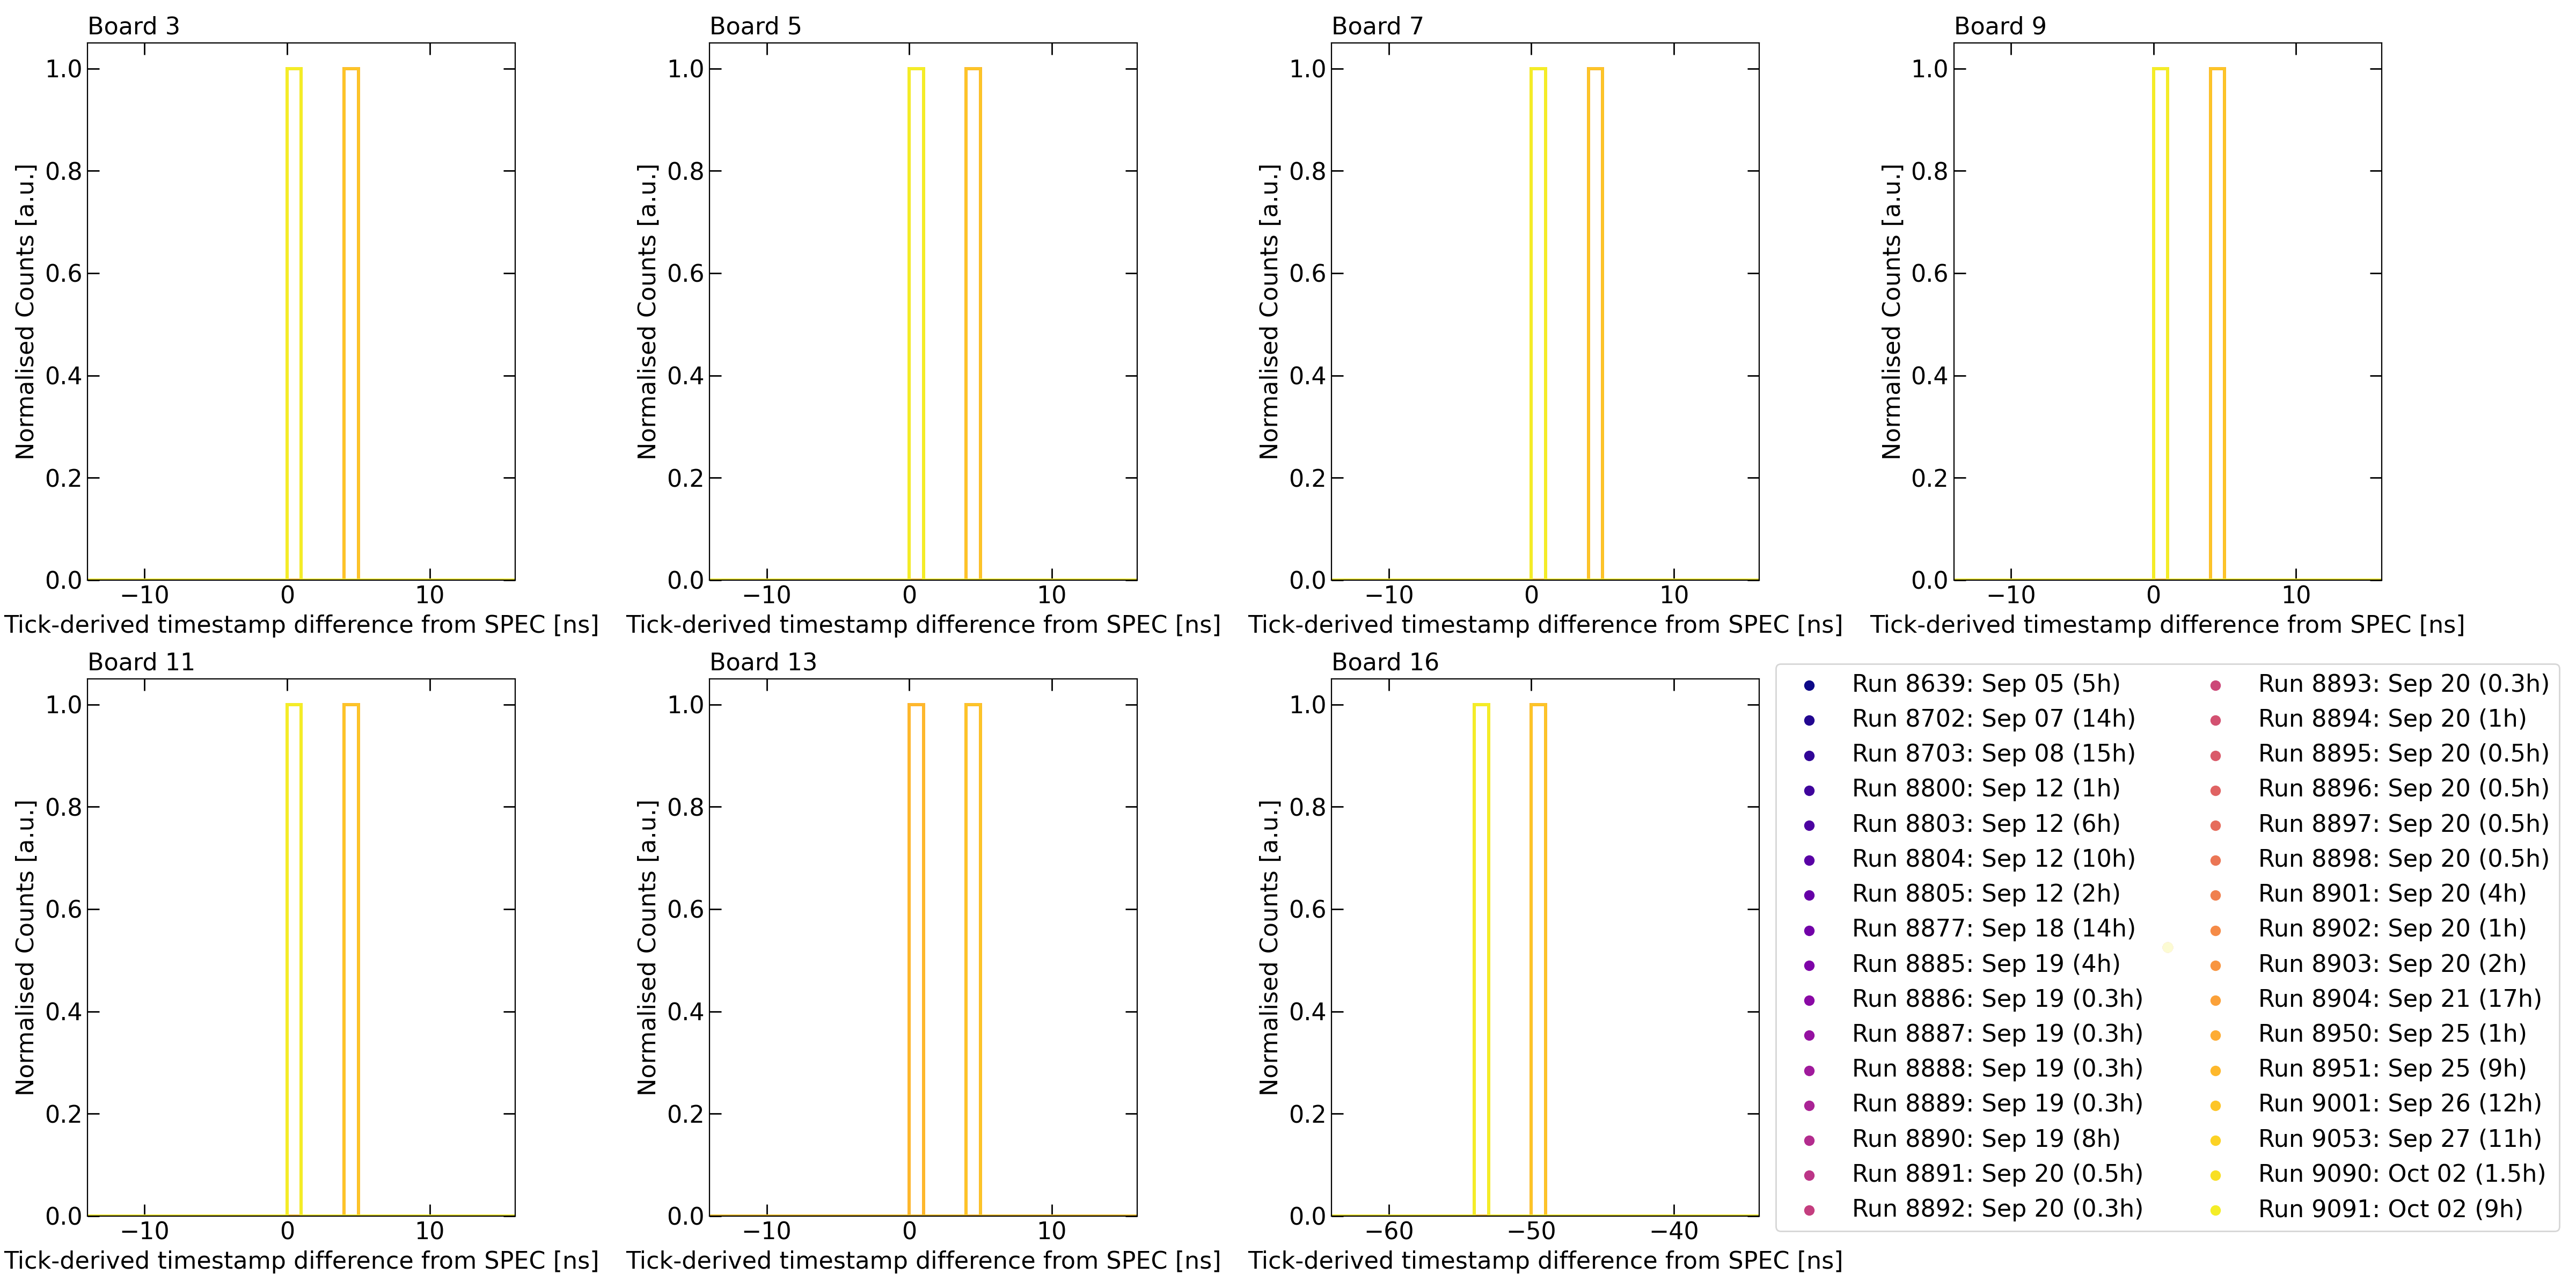
\includegraphics[width=\linewidth]{Tickts_spec_corrEbyE}
\caption{After correction event by event}
\label{subfig:Tickts_spec_corrEbyE}
\end{subfigure}
\vspace{0.5cm}
\begin{subfigure}[h]{1.00\linewidth}
\centering    
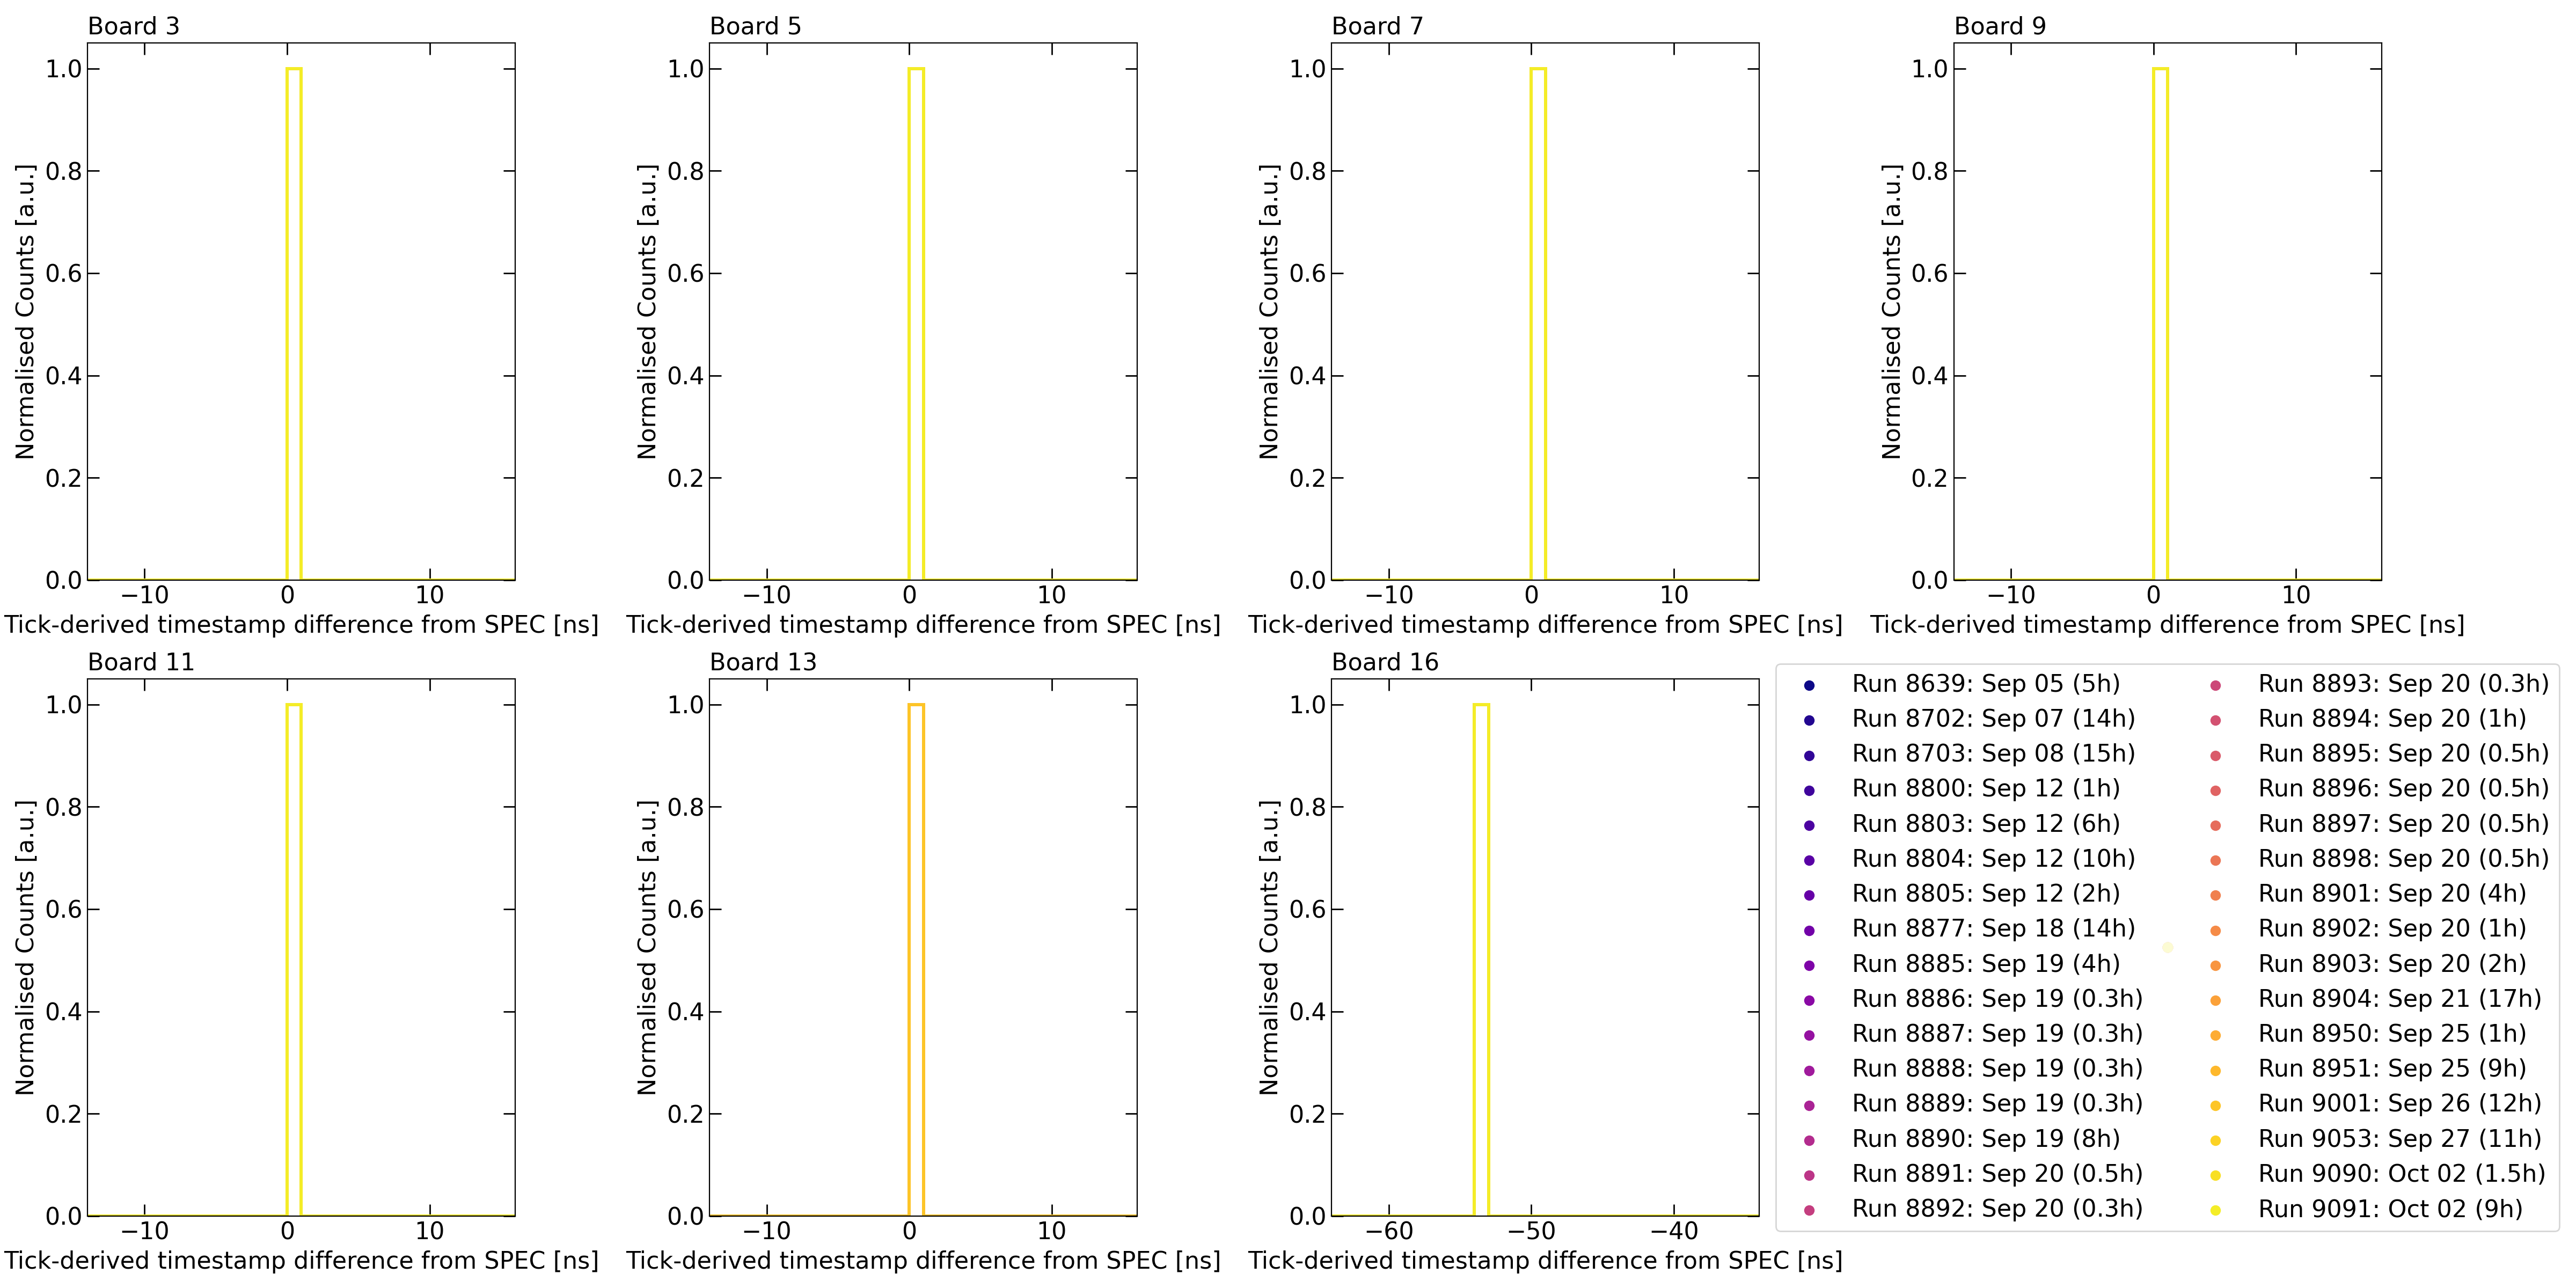
\includegraphics[width=\linewidth]{Tickts_spec_corrRbyR}
\caption{After correction run by run}
\label{subfig:Tickts_spec_corrRbyR}
\end{subfigure}%

\caption[Results of Clock Jittering Correction]{
Differences in trigger timestamps between CAEN digitisers and the SPEC-TDC at each correction step.
}
\label{fig:Tickts_spec_corr}
\end{figure}

This clock jittering study presented here resulted in a new hardware implementation at SBND.
This includes to digitise the trigger signal in channel 15 of every CAEN digitiser as this will provide the necessary timing information for downstream jittering correction.
An additional CAEN digitiser was also installed specifically for digitising beam signals.
It will digitise waveforms of important timing signals needed by downstream analysis to reconstruct the BNB as demonstrated by the MicroBooNE collaboration \cite{uboone_ns}. 

At the time of writing, the clock setup of CAEN digitisers have changed.
Further consultation with the CAEN manufacturer led to a new clock synchronisation scheme.
A 6.25 MHz clock is now distributed in a fan out mode to every digitiser.
Even though it is a lower frequency than 10 MHz, it is a multiple of both the trigger clock (125 MHz) and the sampling clock (500 MHz) so that they can be in phase with each other.
The same clock synchronisation study was performed and the digitised trigger waveforms showed a good agreement to the SPEC-TDC within 1 ns.
This configuration shows an improvement in clock synchronisation and stability than the two methods explored in Section \ref{subsec42PMT}.    
Additionally, digitised waveforms trigger signals, as shown in Fig. \ref{fig:trig_wfm} and \ref{fig:jitterCorr}, were found to be saturated. 
Hardware attenuators were installed, followed by an adjustment of the waveform baseline.
This ensures to capture of the full shape of the trigger waveforms without damaging the digitisers.

%********************************** %Third Section  **************************************
\section{Concluding Remarks}
\label{sec5Remarks}

The timing system at SBND is outlined, detailing the timing signal distribution to ensure synchronisation across different DAQ subsystems. 
As part of the timing system, the SPEC-TDC module records extra timing information applicable for versatile usages.
The module was used to characterise the timing precision of the CRT readout electronics, which was determined to be $\mathcal{O}$(2 ns).
This resolution enables the reconstruction of the beam bucket structure, of which an alternative reconstruction using the T0 timestamps with the SPEC-TDC timing information was demonstrated.
Most importantly, the module was used to examine the clock synchronisation of CAEN digitisers responsible for sampling PMT signals.
This work lead to a clock scheme as well as a correction method to account for clock jittering.
This is a crucial correction to ensure that PMT waveforms are synchronised at the nanosecond level to necessitate the reconstruction of the beam bucket with a high timing resolution.
In the following, Chapter \ref{ChapterCalib} focuses on the calibration of the TPC of SBND, which is another essential step to pin down detector effects affecting high precision physics measurements.

%The event building process relies heavily on precise timing synchronization across these subsystems, achieved through the implementation of the WR timing system.

%Each readout electronic device is synced with a PPS signal derived from the WR devices, ensuring that the timestamps of recorded events from each hardware component align with the frame of reference relative to the PPS signal.

%since the original plan was to digitise beam signals in channel 15.
%The new CAEN digitiser will be used solely for recording beam signals such as the BES and RWM signal.
%The installation of the new hardware setup was carried out by the author during her time at Fermilab and this is photographed in Fig. \ref{fig:pdsR0}.
%The daisy chain clock scheme is chosen, and channel 15 of every digitiser is input with the trigger signals to digitise the waveforms.
%The waveform will contain necessary information for jittering correction in downstream analysis.

%Photograph of the PMT readout electronics crate after the proposal is shown in Fig. \ref{fig:pdsR0}, housing 8 CAEN digitisers on the left for digitising the PMTs, and a new CAEN digitiser on the right for digitising the beam signals.
%\begin{figure}[htbp!] 
%\centering    
%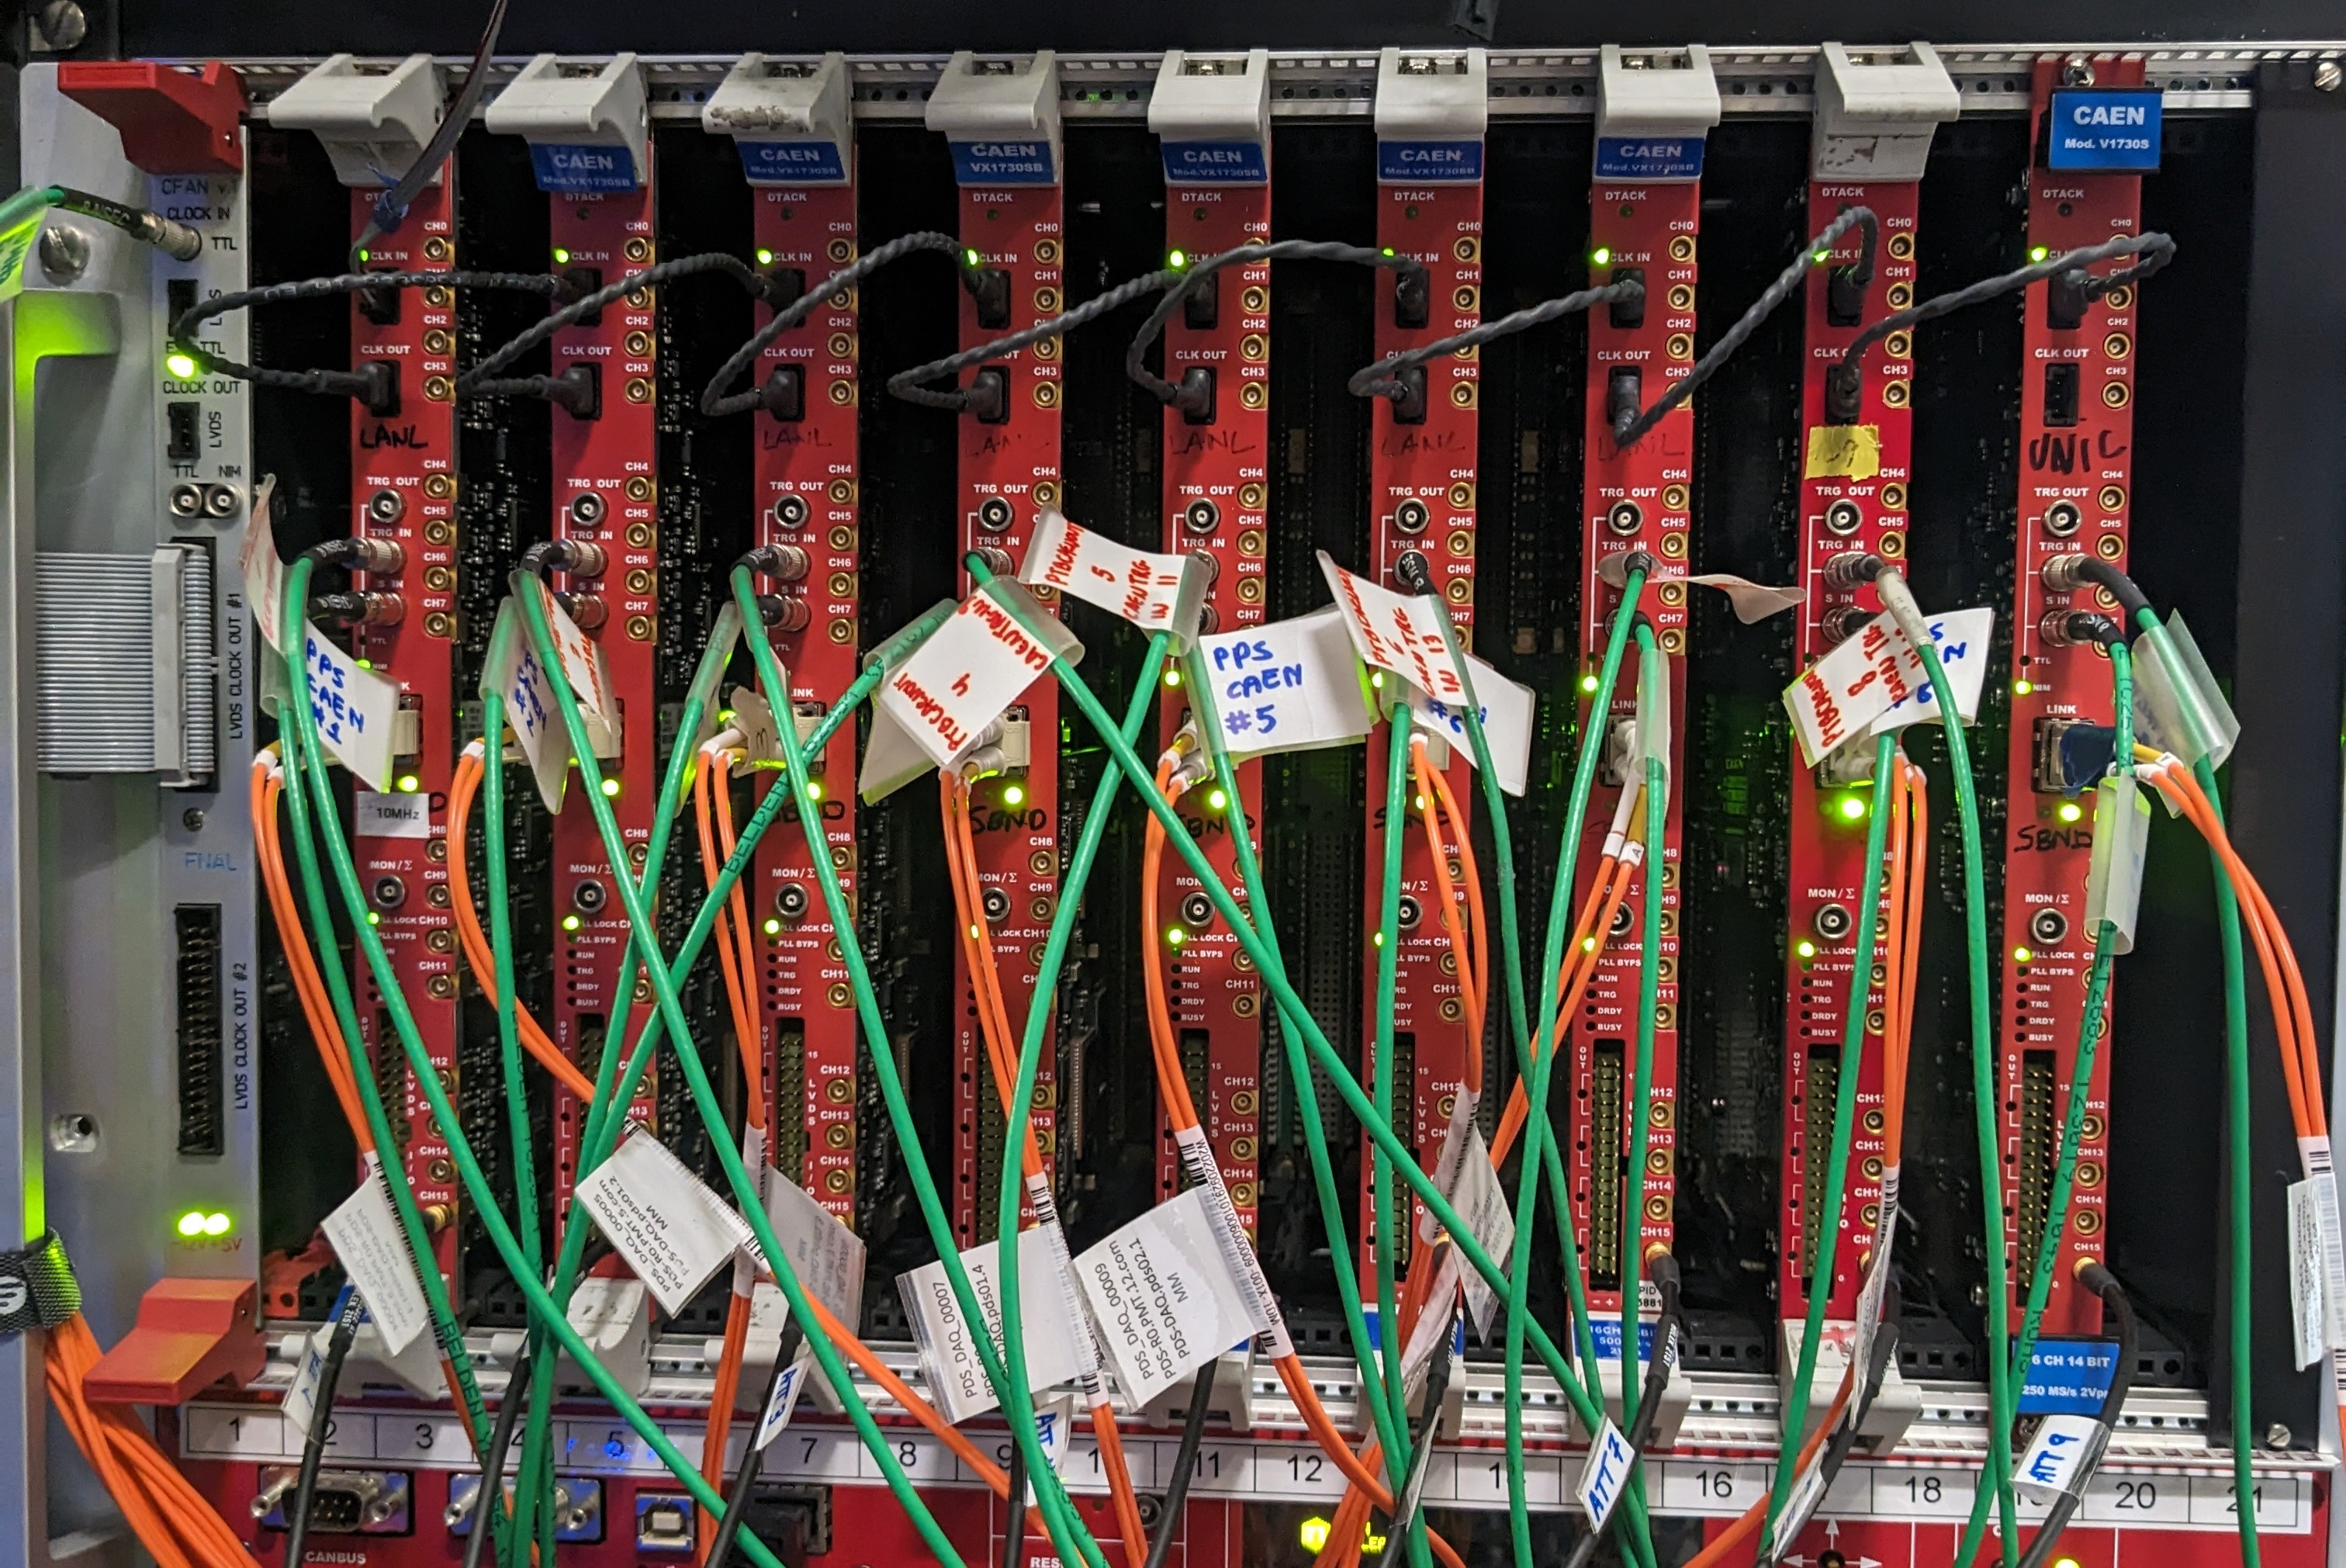
\includegraphics[width=0.6\textwidth]{pds_r0}
%\caption[pdsR0]{
%Photograph of the PMT readout crate.
%}
%\label{fig:pdsR0}
%\end{figure}

%The purpose of this was also to test the stability of the synchronisation of the daisy chain and its impact on the resolution of the produced timestamps.
%The jittering correction to the tick-derived timestamp was applied in steps of event by event, followed by run by run.
%This results in perfect synchronisation across all digitisers and with respect to the PPS signal.
%Board 16 is an exception due to having different firmware. 
%This jittering correction workflow still reveals the amount of correction for this board, which is -54 ns. 
%An additional correction step can be taken to account for time synchronisation across digitisers with different firmwares. 
%The result after the process is demonstrated in Fig. \ref{fig:daisychainCALIB}, showing that every digitiser has the same timestamp and digitises the trigger signal at the exact same tick position on the waveform.As a result, the timestamps of the tick value on the rising edge of trigger signals, or the tick-rived timestamps, are identical across all 8 CAEN digitisers.

%In this configuration, on top of being timestamped, the trigger signal is also digitised as a waveform. 
%In this set up, the 1 Hz trigger is produced from the PTB, and input into the TRG-IN channel of each CAEN for simultaneous triggering.
%The timestamp of the trigger is embedded in the Trigger Time Tag object.
%The trigger is also propagate to a fan out module, and input into channel 15 of every CAEN digitiser.
%The waveform of the trigger signals is expected to be digitised simultaneously. 

%As demonstrate in Fig. \ref{fig:TTTDiagram}, the TTT object is the timestamp of the last tick of waveform, and thus, this provides the timing information to construct the timing of the waveform.
%From the manuals of the digitiser, it is indicated that the trigger clock and the ADC sampling clock are synchronised with respect to each other.
%Monitoring these effects during the commissioning period is necessary to understand the impacts of the clock drift."

%\begin{figure}[htbp!] 
%\centering    
%\includegraphics[width=0.85\textwidth]{digitise_ftrig}
%\caption[digitiseFTRIG]{
%The set up for study the synchronisation of the CAEN digitisers and their timing resolution.
%}
%\label{fig:digitiseFTRIG}
%\end{figure}


%two different modes to compare timestamp
%This set up presents two types of timestamps produced by the CAEN digitiser.
%As illustrated in Fig. \ref {fig:TTTDiagram}, one timestamp is derived from the TTT value produced by the trigger clock of the CAEN digitiser.
%These timestamps were examined in the synchronisation study in section \ref{subsec42PMT}.
%This type of timestamp is now referred as the TTT-derived timestamp.
%Given that the waveform of the trigger signal is now digitised, one can determine the rising edge of the trigger signal.
%This gives a tick value on the waveform and thus, the timestamp associated to this tick which can be derived from the TTT value.
%This type of timestamp is referred as the tick-derived timestamp, since this timestamp requires the knowledge of the tick position of the trigger on the waveform as well as the TTT value.
%Both these timestamps are compared against the SPEC-TDC timestamps of the trigger signals, to the same reference frame at which the trigger leaves the PTB front face.
%Cable length corrections were also applied.

%\begin{figure}[htbp!] 
%\centering    
%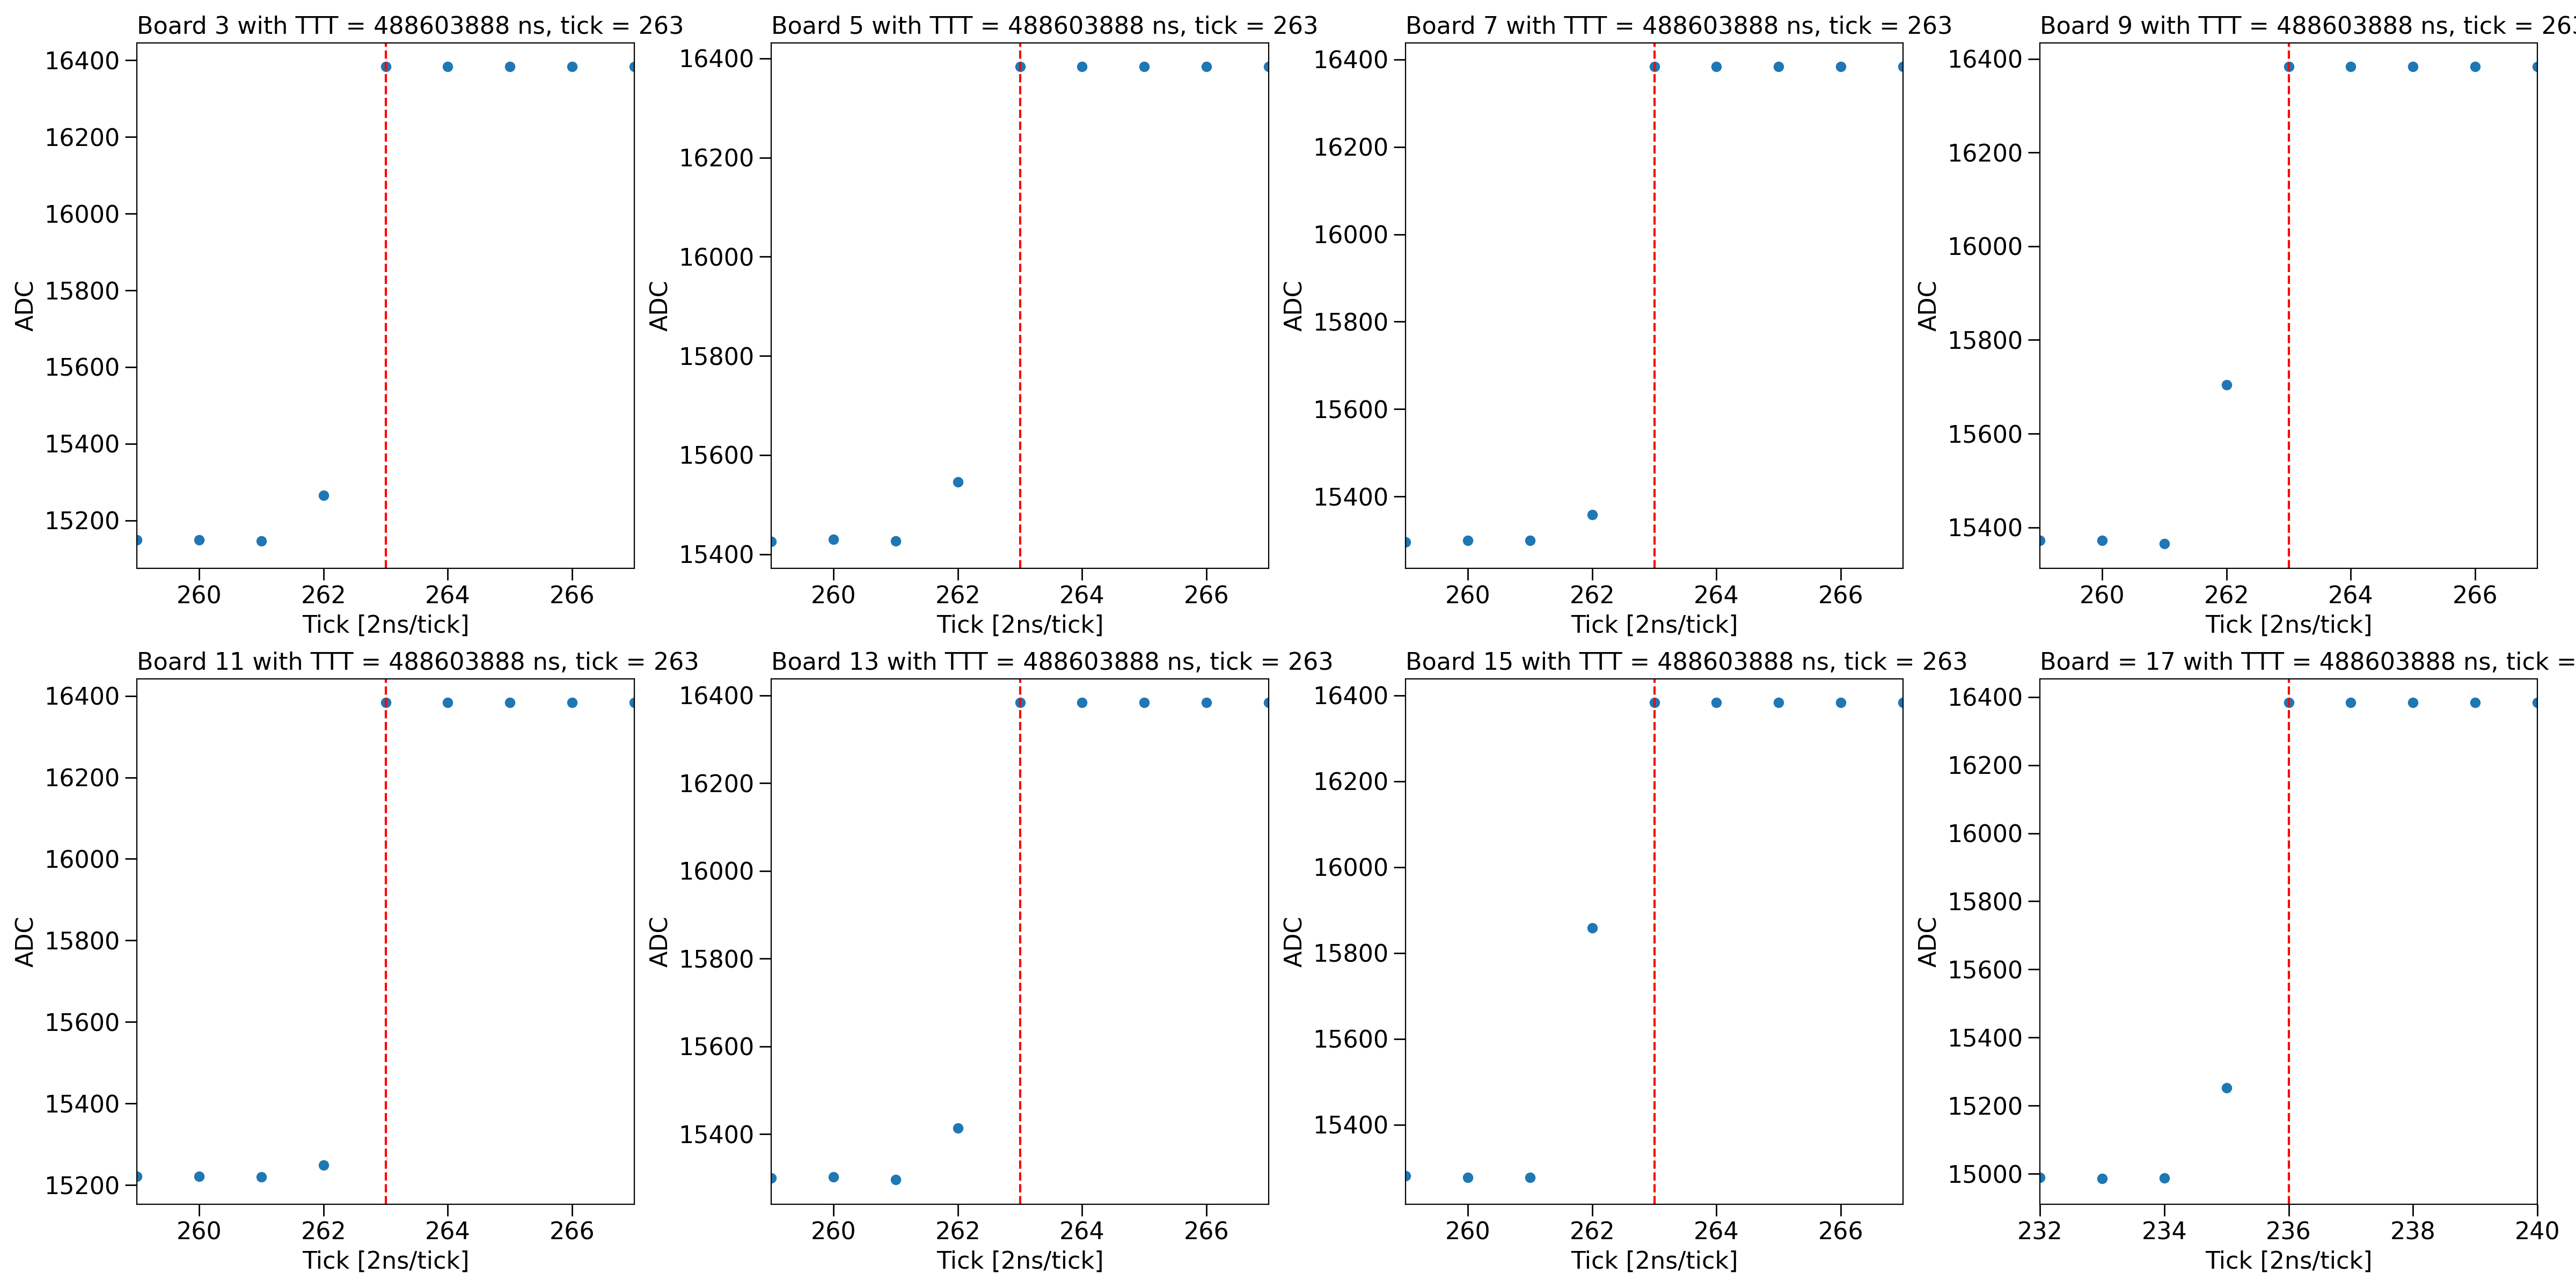
\includegraphics[width=1.0\textwidth]{daisychain_calib}
%\caption[daisychainCALIB]{
%After the daisy chain calibration, the waveforms of the simultaneous triggers are plotted to check for synchronisation.
%The TTT values associated with the each waveform are identical, showing that the digitisers receive triggers at the same time.
%The waveforms of the triggers are zoomed around the rising edge, showing the identical tick value of the rising edge, showing that all the boards also digitise the trigger at the same time.
%Board 17 is an exception because it has a different firmware compared to the rest of the digitisers and digitises the waveform slightly different.
%}
%\label{fig:daisychainCALIB}
%\end{figure}

%\begin{figure}[htbp!]
%
%\begin{subfigure}[h]{1.00\linewidth}
%\centering    
%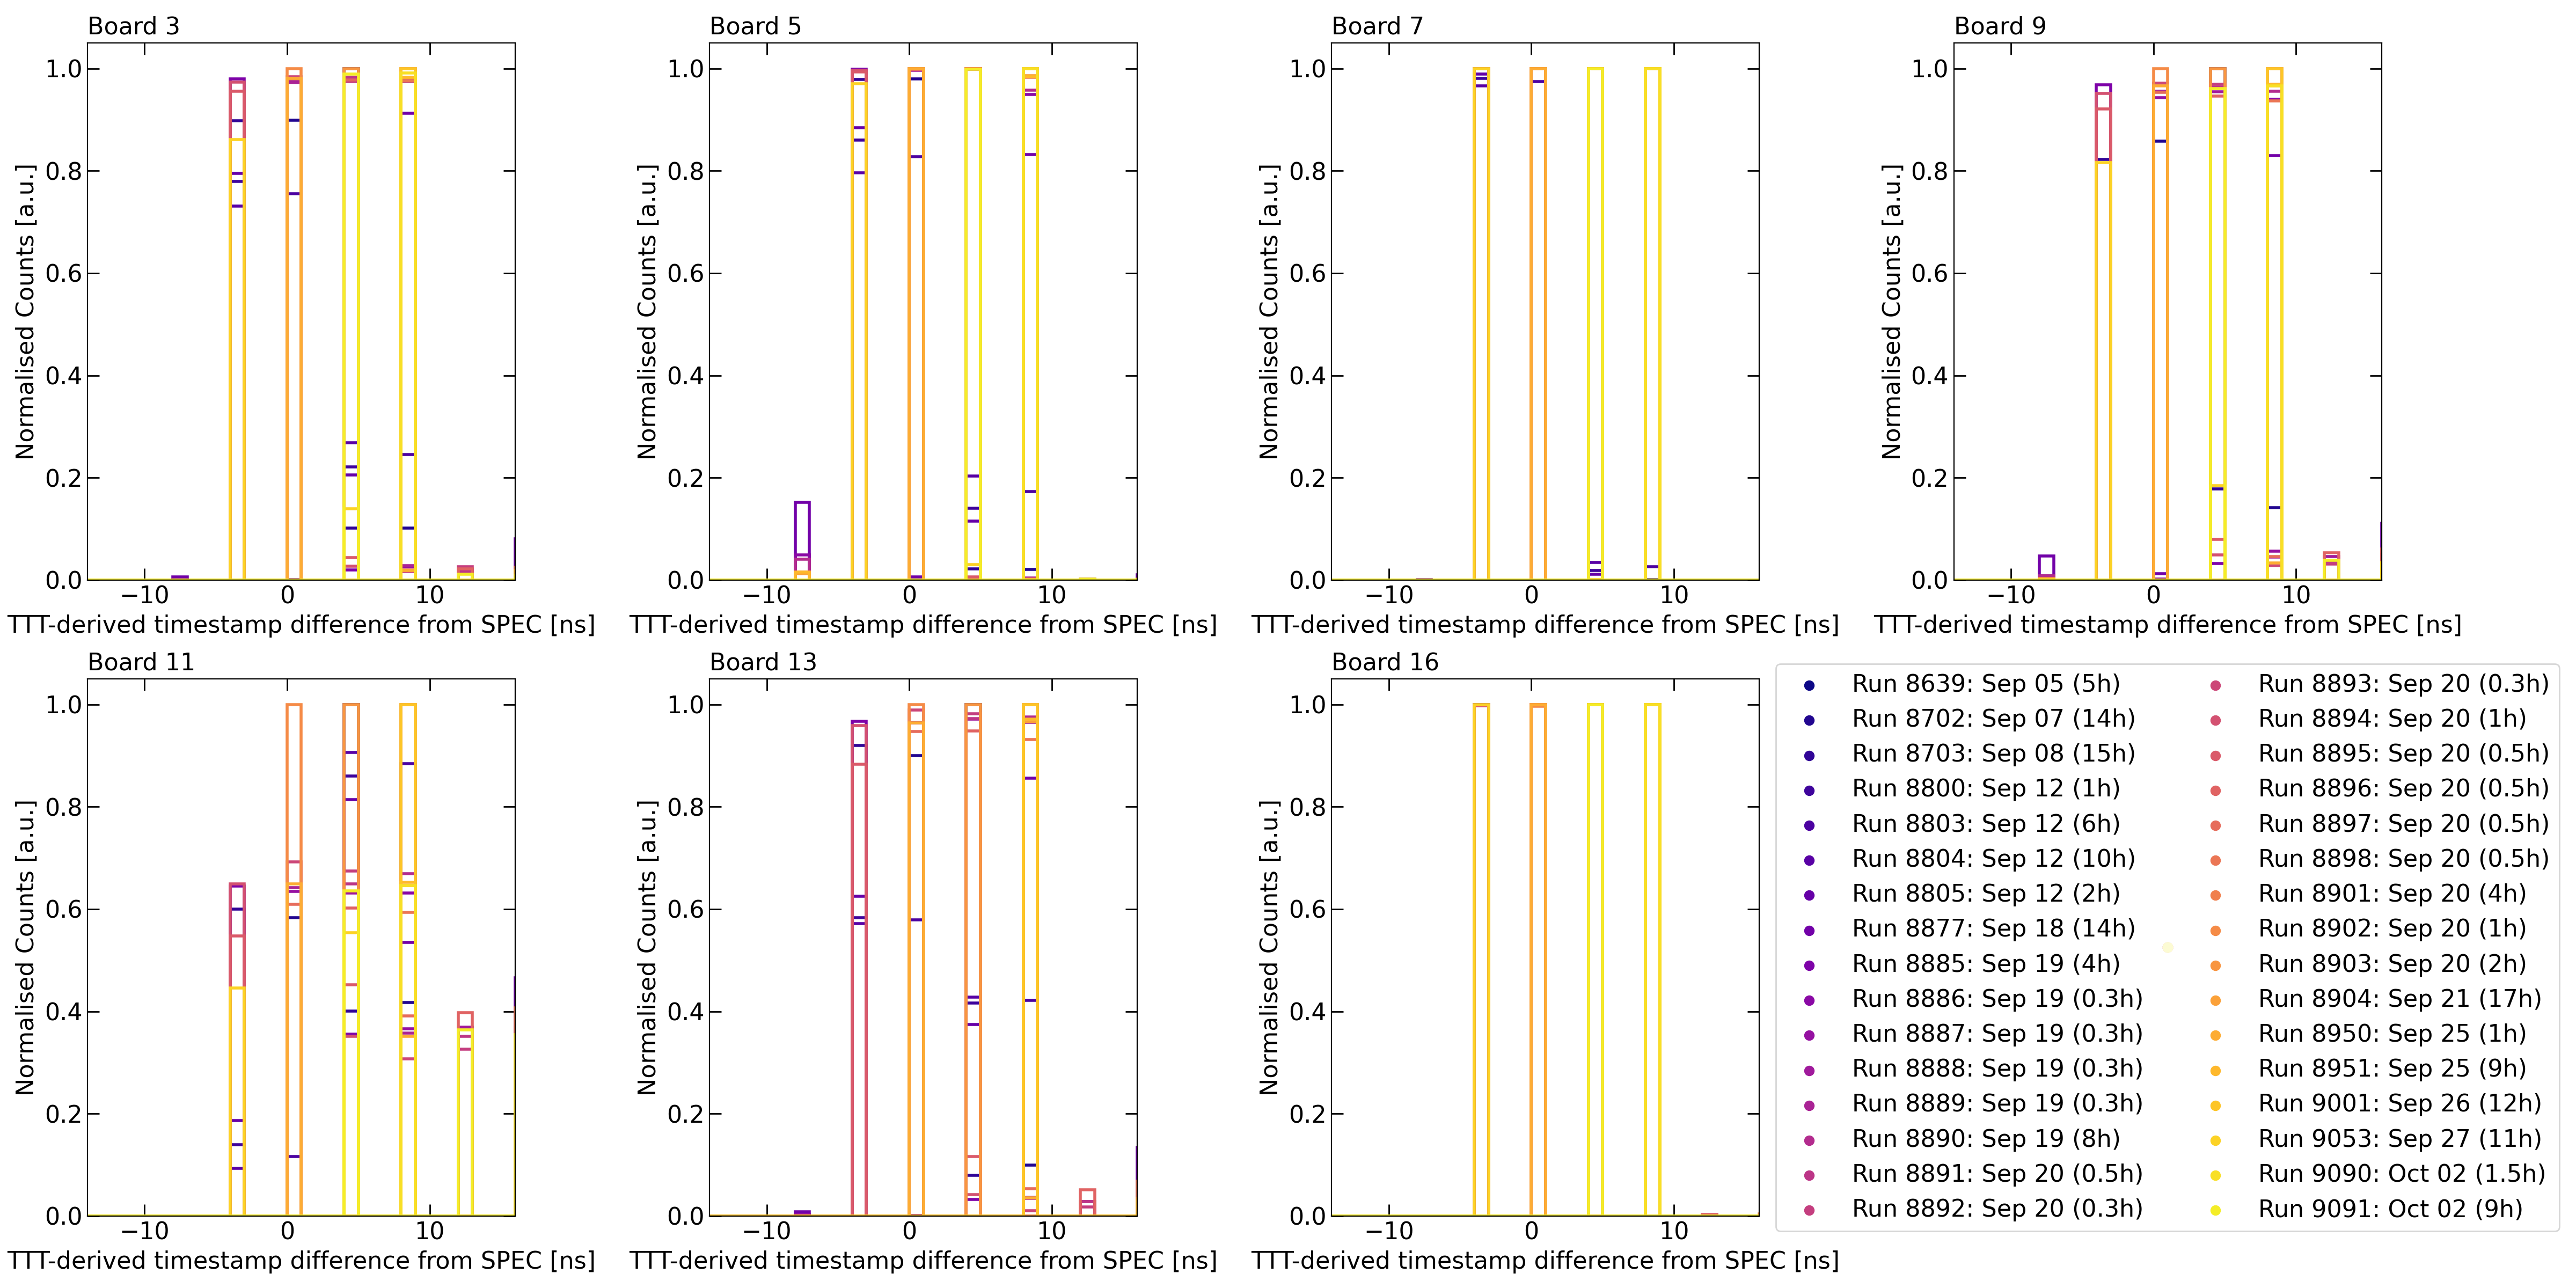
\includegraphics[width=\linewidth]{TTTts_spec}
%\caption{TTT-derived timestamps}
%\label{subfig:TTTts_spec}
%\end{subfigure}
%
%\hfill
%\begin{subfigure}[h]{1.00\linewidth}
%\centering    
%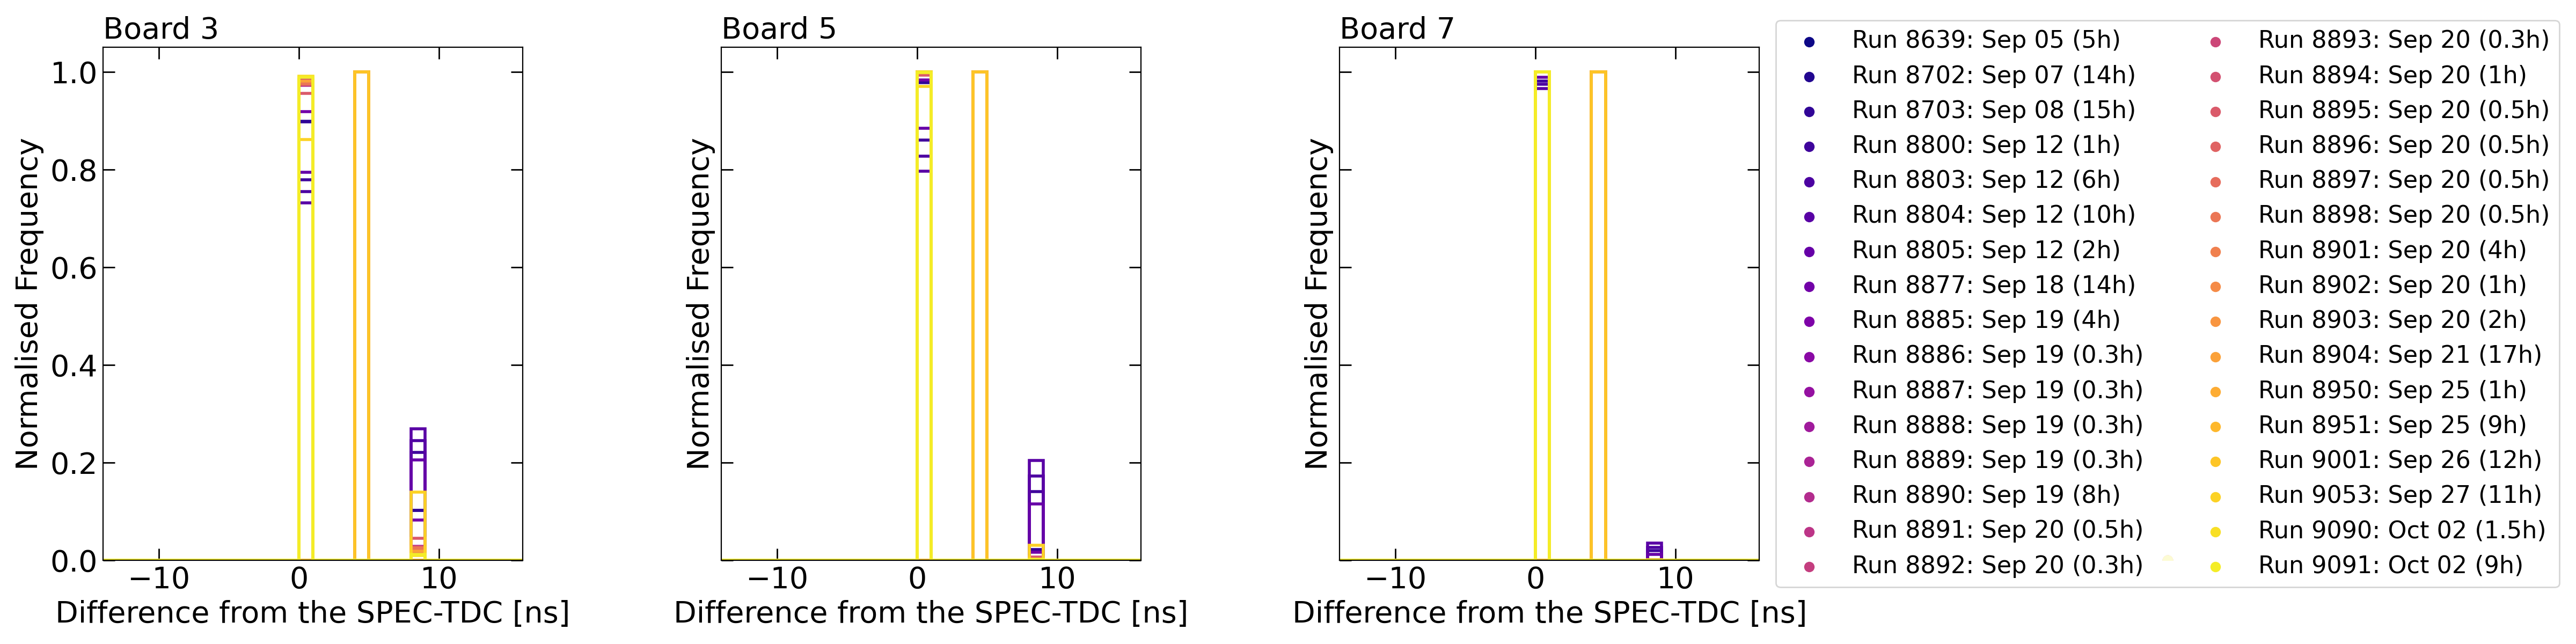
\includegraphics[width=\linewidth]{Tickts_spec}
%\caption{Tick-derived timestamps}
%\label{subfig:Tickts_spec}
%\end{subfigure}%
%
%\caption[TTTtsTickts]{
%The two timestamps distributions generated by the CAEN digitisers, compared against the SPEC-TDC timestamps.
%The TTT-derived timestamps show a large spread up to 24 ns whilst the Tick-derived timestamps show a much smaller spread of only 8 ns.
%}
%\end{figure}

%TTT timestamps
%The TTT-derived timestamps distribution is plotted in Fig. \ref {subfig:TTTts_spec} for 7 CAEN digitisers, compared against the SPEC-TDC timestamps.
%This distribution shows a large spread up to 24 ns, which indicates that TTT-derived timestamp has a variation larger than what is stated in the manuals, that the trigger clock resolution is 16 ns.
%The tick-derived timestamps distribution is plotted in Fig. \ref {subfig:Tickts_spec}.
%This distribution, however, shows a much small spread of only 8 ns.

%To understand the differences between the two types of timestamps, the tick position of the rising edge of the trigger waveform is also plotted in Fig. \ref {fig:TickSPEC}.
%The distribution shows a large spread up to 5 ticks, equivalent to 10 ns.
%This illustrates that the CAEN digitiser does not consistently digitise the trigger waveform, causing variations in the tick position of the rising edge between different events, run and digitisers.
%This implies that not only can the trigger clock of the CAEN digitiser jitter, but its ADC sampling clock can also fluctuate, potentially introducing additional smearing.

%\begin{figure}[htbp!]
%\centering    
%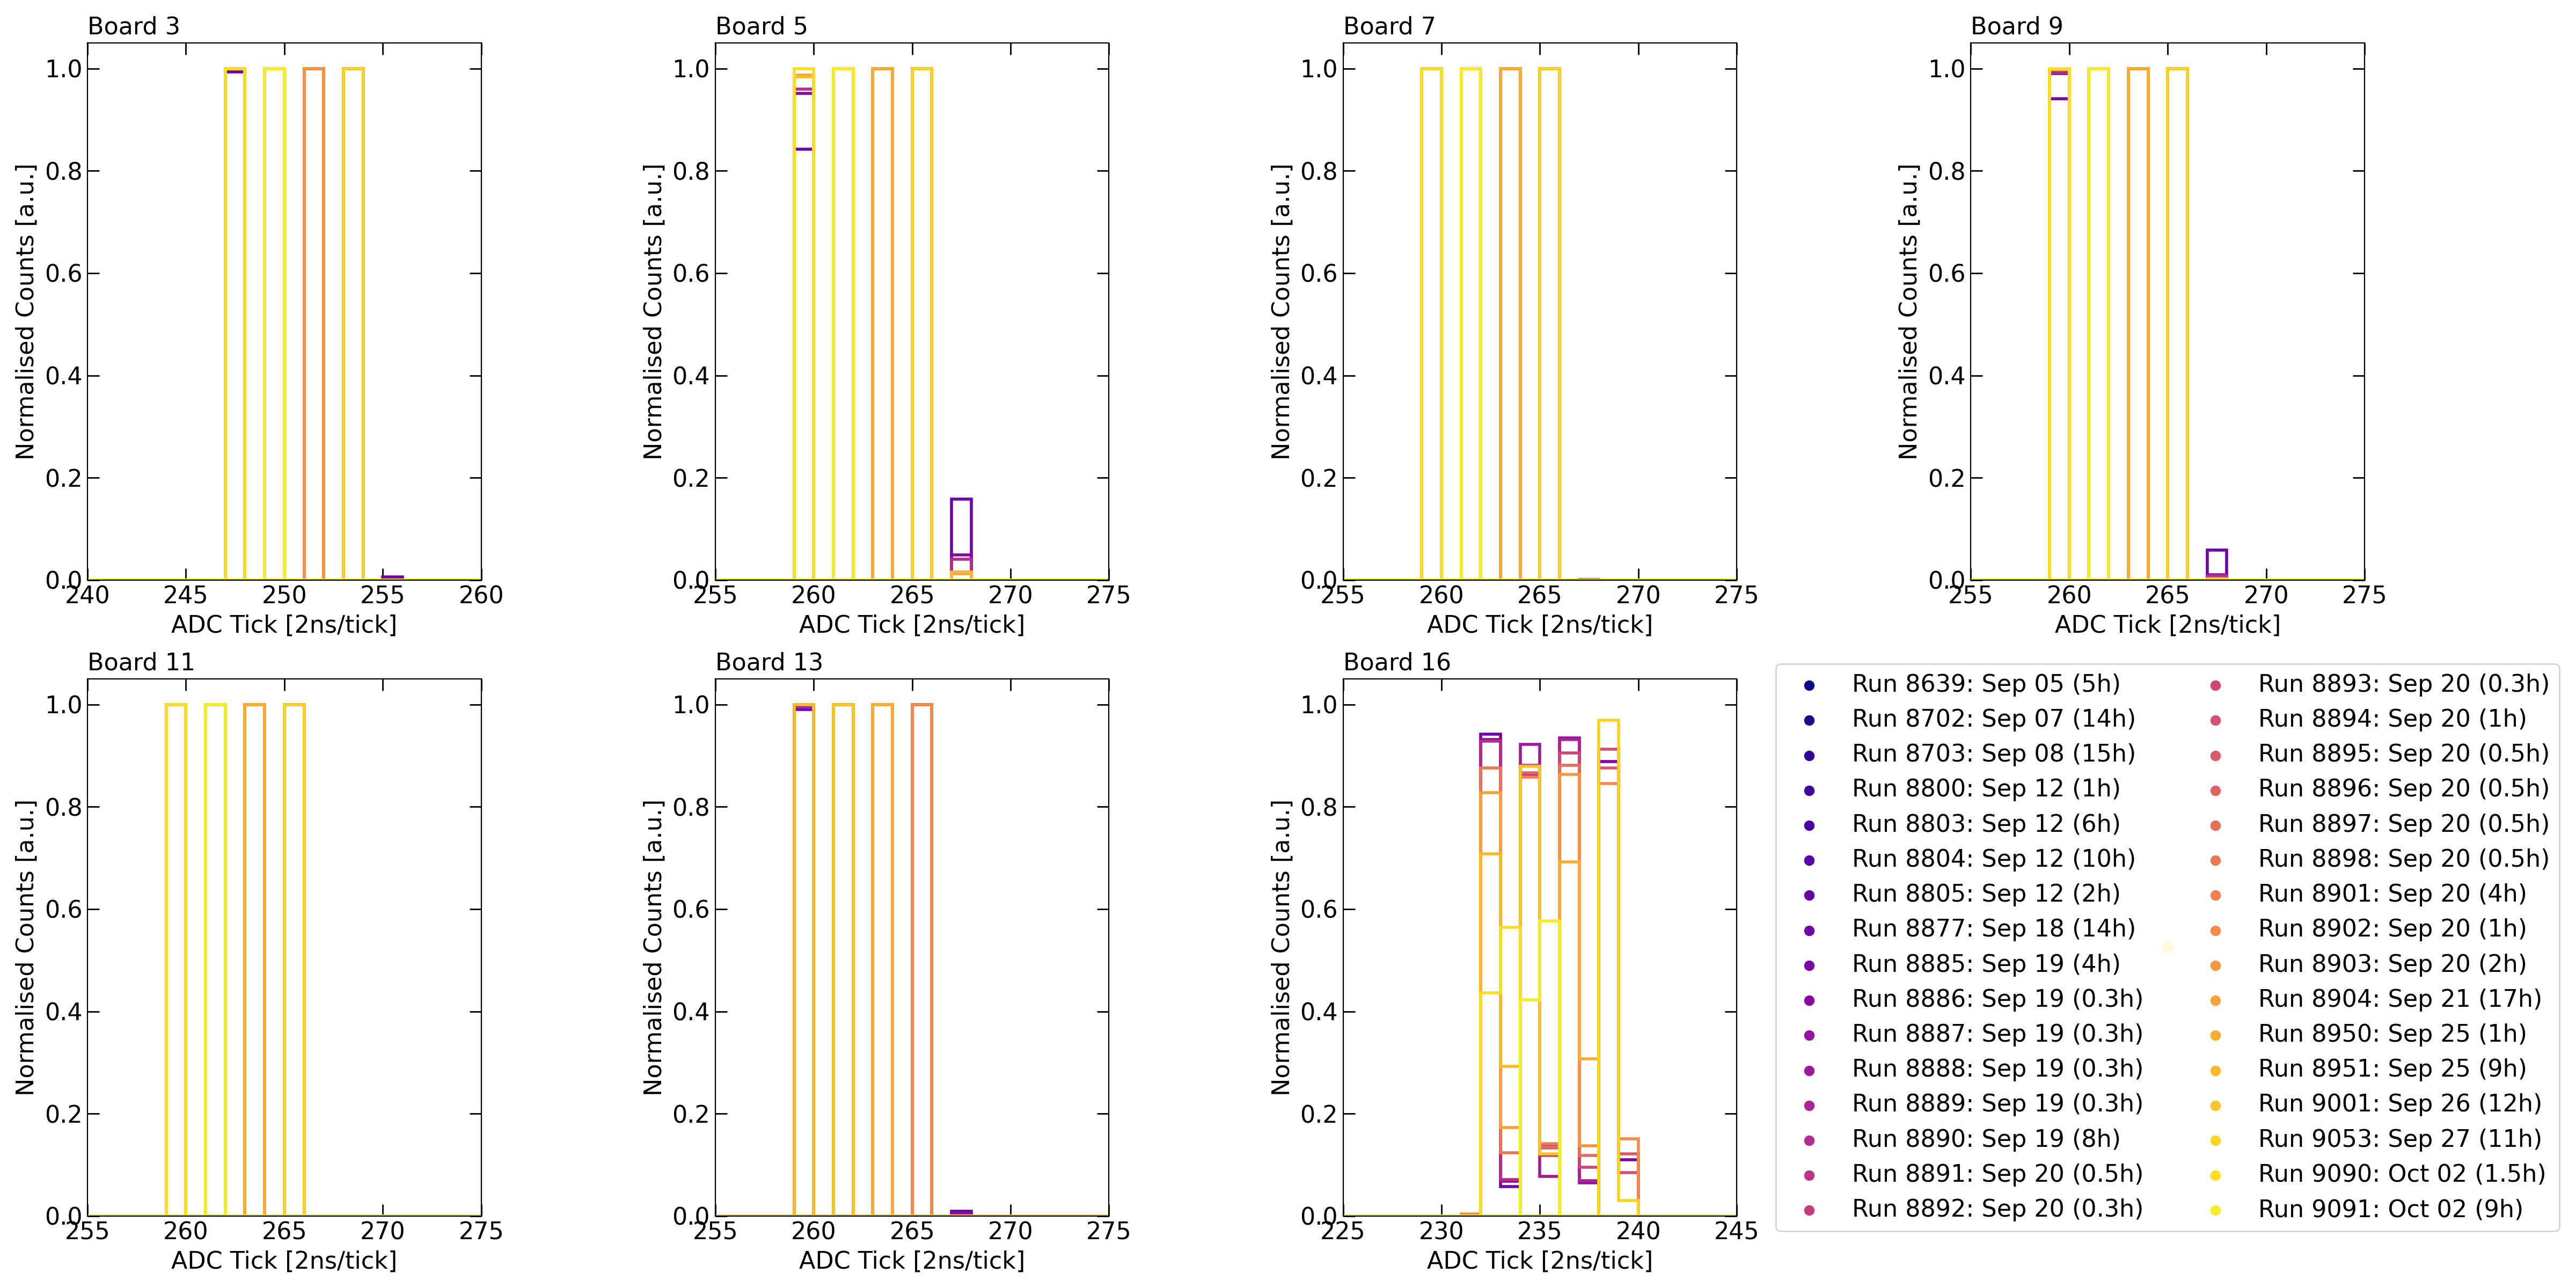
\includegraphics[width=\linewidth]{Tick_spec}
%\caption[TickSPEC]{
%The distribution of the tick value of the rising edge of the trigger waveforms has variation up to 5 ticks, equivalent to 10 ns. 
%This demonstrates that the ADC sampling clock of the CAEN digitiser can also jitter.
%}
%\label{fig:TickSPEC}
%\end{figure}

%The CAEN manuals highlight that the trigger clock and the ADC sampling clock are correlated to each other, and this is reflected in the fact that the TTT value points to the last tick of the wave form.
%The CAEN digitiser was designed on purpose to have the trigger clock in synchronised with the ADC sampling clock, so that the trigger clock can track and absorb the jittering of the ADC sampling clock.
%This explains the 24 ns spread of the TTT-derived timestamps since it contains the smearing from both the trigger and the ADC sampling clocks.
%Meanwhile, the tick-derived timestamps distribution shows a much smaller spread of 8 ns, since tht timestamp was produced using both the TTT value and tick value, resulting in a high level of precision.
